\documentclass{article}
% preamble
  \usepackage[letterpaper, top=1in, bottom=1in, left=1in, right=1in]{geometry}
  \usepackage[utf8]{inputenc}
  \usepackage[english]{babel}
  \usepackage{tikz-cd, lipsum, bm, dcolumn}
  \usetikzlibrary{arrows}
  \usepackage{amsmath, amssymb, amsthm, mathrsfs, mathtools, centernot, hyperref, fancyhdr, lastpage}
  \usepackage{extarrows, esvect, esint, pgfplots}
  \pgfplotsset{compat=1.18}

  \setlength{\parindent}{0pt} % set no indent
  \hfuzz=5.0pt % ignore overfull hbox badness warnings below this limit

  \DeclareMathOperator{\Tr}{Tr}
  \DeclareMathOperator{\Sym}{Sym}
  \DeclareMathOperator{\Span}{span}
  \DeclareMathOperator{\std}{std}
  \DeclareMathOperator{\Cov}{Cov}
  \DeclareMathOperator{\Var}{Var}
  \DeclareMathOperator{\Corr}{Corr}


  \theoremstyle{definition}
  \newtheorem{theorem}{Theorem}[section]
  \newtheorem{proposition}[theorem]{Proposition}
  \newtheorem{lemma}[theorem]{Lemma}
  \newtheorem{example}{Example}[section]
  \newtheorem{corollary}{Corollary}[theorem]
  \theoremstyle{remark}
  \newtheorem*{remark}{Remark}
  \theoremstyle{definition}
  \newtheorem{definition}{Definition}[section]
  \renewcommand{\qed}{\hfill$\blacksquare$}
  \renewcommand{\footrulewidth}{0.4pt}% default is 0pt

  \renewcommand{\thispagestyle}[1]{}

\begin{document}
\pagestyle{fancy}

\lhead{Stochastic Processes}
\chead{Muchang Bahng}
\rhead{\date{Spring 2023}}
\cfoot{\thepage / \pageref{LastPage}}

\title{Stochastic Processes}
\author{Muchang Bahng}
\date{Spring 2023}

\maketitle
\tableofcontents 
\pagebreak 

\section{Introduction}

  Ordinary differential equations model deterministic systems that can be solved exactly through integration. For example, consider the population model determined by a linear DEQ 

    \[\frac{d N} {dt} = \alpha(t) N (t)\]

  where $N$ is the population size and $\alpha$ is a growth rate. Then, we can solve with analysis by integrating the following with a change of basis

  \begin{align*}
    \int \frac{1}{N(t)} \frac{dN}{dt} \,dt = \int \alpha(t) \,dt \iff \int \frac{1}{N} \, dN = \int \alpha(t) \,dt \\
    & \iff N(t) = C \exp \bigg( \int \alpha (t) \,dt \bigg) 
  \end{align*}
  
  This classical exponential growth model is not only continuous, but \textit{smooth}, and it is this smoothness that allows us to do calculus on it. But more realistic models will have noise, which can be modeled by a random variable. Let $\alpha = r + \eta$, where $r$ is the deterministic term and $\eta$ is the random term. Then, integrating gives us 

    \[\frac{dN}{dt} = \big( r(t) + \eta(t) \big) N(t) \iff \int \frac{1}{N} \frac{dN}{dt} \,dt = \int r(t) \,dt + \int \eta(t) \,dt\]
    
  The first integral can be evaluated, but classical calculus does not allow us to integrate the random part. This is where stochastic calculus is needed. Now recall from probability that a random variable over a probability space $(\Omega, \mathcal{F}, \mathbb{P})$ is simply a $\mathcal{F}$-measurable function $X$. As some warm up exercises, let us prove a few examples. 

  \begin{example}[Class 1] 
    
  \end{example}

  \begin{example}[Class 2]
    
  \end{example}

  \begin{definition}[Stochastic Process]
    A \textbf{stochastic process} is a collection of random variables indexed by time $\{X_t\}_{t \in T}$ with their respective measures $\rho_t$. 

    \begin{enumerate}
      \item If $T$ is countable (usually integers), then it is called a \textbf{discrete-time} stochastic process. 
      \item If $T$ is continuous, then it is called a \textbf{continuous-time} stochastic process. 
    \end{enumerate}

    It is also good to think of it as a probability distribution over a space of paths. 
  \end{definition}

  We first start off with Markov processes. We can divide them into four kinds, depending on whether we are using discrete or continuous time, and whether we are using discrete or continuous state space. Since process over continuous state space is a natural generalization of those in a discrete one, we only distinguish between the times. When talking about continuous time, there are additional operators we must introduce, such as generators. Before we go any further, I would like to mention that these set of notes will write down the transition matrices of Markov chains as left-stochastic matrices, as they are usually written in convention. Therefore, a transition matrix would look like 

    \[\mathbb{P} = \begin{pmatrix} P(1, 1) & \ldots & P(d, 1) \\ \vdots & \ddots & \vdots \\ P(1, d) & \ldots & P(d, d) \end{pmatrix} \]

  where $P(i, j)$ represents the probability of transition from state $i$ to state $j$. Therefore, the rows must sum to $1$. I use this notation because it is consistent with when we are working with Markov processes over general measurable state spaces. Note that we will denote in math font general objects and operators ($X_t, \rho_t, P_s, \pi$) and their realization as vectors and matrices in bold font ($\boldsymbol{\rho_t}, \mathbf{P_s}, \boldsymbol{\pi}$). 

  \subsection{Transitioning from Discrete to Continuous State Space}

    Let us remind ourselves of the definitions involving Markov chains over a discrete state space. Let $X_t$ be the state at time $t$. The discrete distribution of $X_t$ can be represented as a column vector $\boldsymbol{\rho_t}$, where $\boldsymbol{\rho_t} (i) = \mathbb{P}(X_t = i)$, and we can calculate the distribution of $X_{t + s}$ as 

      \[\boldsymbol{\rho_{t + s}}^T = \boldsymbol{\rho_{t}}^T \boldsymbol{P_s} \]

    where $\boldsymbol{P_s}$ is a stochastic matrix. Note that representing a discrete measure on discrete $S = \{1, \ldots, d\}$ with a vector really just a notational convenience for computations. We must properly distinguish the three: 

    \begin{enumerate}
      \item the actual state $X_t$ 
      \item the probability distribution $\rho_t$, which is a measure 
      \item the PMF vector $\boldsymbol{\rho_t}$, which is just a convenient representation of $\rho_t$ in the way that 
      \[\boldsymbol{\rho_t} (i) = \rho_t (\{i\}) = \mathbb{P}(X_t = i)\]
      That is, the $i$th element is just the measure on the singleton set $\{i\} \in \mathcal{S} = 2^S$. 
    \end{enumerate}

    The PMF vector $\boldsymbol{\rho_t}$ is really just a way to describe $X_t$ and its distribution, which is redundant. Furthermore, when we try to describe states $X_t$ in general measure spaces $(S, \mathcal{S})$, we cannot think of it as a vector anymore. This is not a problem in even countable spaces since we can just assign $\boldsymbol{\rho_t} (i) = \mathbb{P}(X_t = i)$ in a finite space, but for uncountably infinite spaces we cannot do this. Therefore, we must have some measurable \textbf{function} $f: S \rightarrow \mathbb{R}$ that extracts this kind information from $X_{t}$. Therefore, we must really work with the following: 

    \begin{enumerate}
      \item the actual state $X_t: (\Omega, \mathcal{F}, \mathbb{P}) \longrightarrow (S, \mathcal{S})$ 
      \item the probability distribution $\rho_t$ of the state $X_t$ 
      \item a collection of $\mathcal{S}$-measurable functions $f: S \longrightarrow \mathbb{R}$ that describes the state 
    \end{enumerate}

    At this point, we are not sure what $f$ is since it seems quite arbitrary. But if we fix some $A \in \mathcal{S}$ and take $f = 1_A$, then $1_A (X_t)$ encodes the information of whether $X_t$ is in $A$ or not. This is quite nice, since now we can think of the PMF vector $\boldsymbol{\rho_t}$ as having components defined by the functions 

      \[\boldsymbol{\rho_t} (i) = 1_{\{i\}} (X_t) = \mathbb{P}(X_t = i)\]

    The following theorem formalizes this concept. 

    \begin{theorem}
      Two random variables $X, Y : (\Omega, \mathcal{F}, \mathbb{P}) \rightarrow (S, \mathcal{S})$ have the same distribution if 

        \[\mathbb{E}[f(X)] = \mathbb{E}[f(Y)]\]

      for all $\mathcal{F}$-measurable $f: S \rightarrow \mathbb{R}$, which can be seen by setting $f = 1_A$ for any $A \in \mathcal{F}$. 

      \begin{align*}
        \mathbb{E}[1_A (X)] = \mathbb{E}[1_A (Y)] & \implies \mathbb{P}(X \in A) = \mathbb{P}(Y \in A) \\
        & \implies \mathbb{P}_X (A) = \mathbb{P}_Y (A)
      \end{align*}
      and so the measure that $X$ and $Y$ pushes forward to $(S, \mathcal{S})$ is precisely the same. This does not mean that they are the same random variable. 
    \end{theorem}

    Let's talk more about $f$ in the discrete case setting. We know that the discrete distributions are represented by a column vector. It is true that every measurable function can be written as a linear combination of simple (indicator) functions, and so in a discrete space $S = \{1, \ldots, d\}$, we can write every $f$ as 

      \[f = \sum_{i \in S} f_i 1_{\{i\}} \]

    which outputs $f_i$ if its input is $i$. We can interpret it as a column vector $\mathbf{f} = (f_1, \ldots, f_d)^T$ . We can see that 

      \[\boldsymbol{\rho_t}^T \mathbf{f} = \begin{pmatrix} \boldsymbol{\rho_t} (1) & \ldots & \boldsymbol{\rho_t} (d) \end{pmatrix} \begin{pmatrix} f_1 \\ \vdots \\ f_d \end{pmatrix} = \mathbb{E}[f(X_t)]\]

    and if $\mathbf{f}$ is any standard unit vector, say $(1, 0, 0)$ with $d = 3$, then

      \[\boldsymbol{\rho_t}^T \mathbf{f}  = \begin{pmatrix} \boldsymbol{\rho_t} (1) & \boldsymbol{\rho_t} (2) & \boldsymbol{\rho_t} (3) \end{pmatrix} \begin{pmatrix} 1 \\ 0 \\ 0 \end{pmatrix}= \mathbb{E}[1_{\{1\}} (X_t)] = \mathbb{P}(X_t = 1)\]

    Therefore, every time we compute $\mathbb{E}[f(X_t)]$, we can think of it in the discrete case as dotting $\boldsymbol{\rho_t}$ with a function vector $\mathbf{f}$ to extract whatever we want from the vector $X_t$. And as we will find out later, the linearity of the stochastic matrix $\mathbf{P_s}$ is analogous to the linearity of the Markov semigroup $P_s$.  

    Therefore, our Markov process is really just some stochastic process $\{X_t\}_{t \geq 0}$ over some measurable space $(S, \mathcal{S})$ with the property that 

      \[\mathbb{P}(X_{t + s} \in A \mid \{X_r \in B_r\}_{r \leq t}) = \mathbb{P}( X_{t + s} \in A \mid X_t \in B_t)\]

    where $A \in \mathcal{S}$, and this captures the discrete case by setting $A = \{j\} \in 2^S$ which gives 

      \[\mathbb{P}( X_{t + s} = j \mid \{X_r = i_r\}_{r \leq t}) = \mathbb{P}( X_{t + s} = j \mid X_t = i_t)\]

    This basically says that the probability that $X_{t + s}$ lying in $A$ is only dependent on its present state $X_t \in B_t$, not the history $\{X_r \in B_r\}_{r \leq t}$. In fact, by using the identity $\mathbb{E}[1_A] = \mathbb{P}(A)$ and setting $f = 1_A$, we can capture this effect for \textit{all} measurable $f: (S, \mathcal{S}) \rightarrow (\mathbb{R}, \mathcal{R})$. Thus, the Markov property now looks like  

      \[\mathbb{E}[f (X_{t + s}) \mid \{X_r \in B_r\}_{r \leq t}] = \mathbb{E}[ f(X_{t + s}) \mid X_t \in B_t]\]

    We don't need to fix the $X_r$'s into sets $B_r$'s and so we can write 

      \[\mathbb{E}[f (X_{t + s}) \mid \{X_r\}_{r \leq t}] = \mathbb{E}[ f(X_{t + s}) \mid X_t]\]


    Now let's talk about this Markov property. It is true that $\sigma$-algebra $\sigma(\{X_r\}_{r \leq t})$ is bigger than $\sigma(X_t)$; the Markov property does not imply that they are the same size. Rather, we should interpret this as the extra information introduced by the bigger $\sigma(\{X_r\}_{r \leq})$ is irrelevant. This is analogous to trying to approximate a function with a pointlessly large $\sigma$-algebra. For example, given a piecewise function $X$ defined on the unit interval $\Omega = [0, 1]$, let $\mathcal{G}$ be the $\sigma$-algebra generated by $[0, 0.5), [0.5, 1]$ and $\mathcal{H}$ be that generated by $[0, 0.25), [0.25, 0.5), [0.5, 0.75), [0.75, 1]$. 

    \begin{center}
      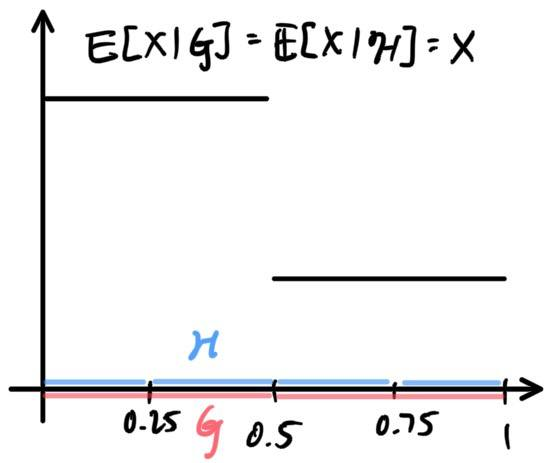
\includegraphics[scale=0.3]{img/pointless_approximation.jpg}
    \end{center}

    Then, we can see that 

      \[\mathbb{E}[X \mid \mathcal{G}] = \mathbb{E}[X \mid \mathcal{H}]\]

    That is, the two random variables are exactly equal, even though $\mathcal{H}$ has more information than $\mathcal{G}$. Note that this is not the law of iterated expectations. This rule does not say that $\mathbb{E}[\mathbb{E}[X \mid \mathcal{G}]] = \mathbb{E}[ \mathbb{E}[X \mid \mathcal{H}]]$; this law is true regardless. Rather, this property is a special property of the function $X$, and therefore the Markov property is a special property of the stochastic process $\{X_t\}_{t \geq 0}$. 

\section{Discrete-Time Markov Processes}

  \begin{definition}[DTMP]
    Let $(\Omega, \mathcal{F}, \mathbb{P})$ be a probability space and $(S, \mathcal{S})$ a measurable space. Then, a homogeneous \textbf{discrete-time Markov process} is a stochastic process $\{X_n\}_{n \in \mathbb{N}}$ which takes values in $S$ (i.e. $X_n: \Omega \rightarrow S$) satisfying the \textbf{Markov property}: for every bounded measurable $f$ and $n \geq 1$, 

      \[\mathbb{E}[f(X_{n + m}) \mid \{X_r\}_{r=0}^n] = \mathbb{E}[f (X_{n + m}) \mid X_n] = (P_m f) (X_n)\]

    Since this is true for all $n$, this process is \textbf{time-homogeneous}. Note that both sides are random variables, and it says that the best estimate of $f(X_{n+m})$ as a function of $\{X_r\}_{r=0}^n$ can be simply expressed as as a function of the current $X_n$. Notice also that we have given a specific label $P_m f$ to the conditional expectation on the right hand side. 
  \end{definition}

  Since every $X_n$ has distribution $\rho_n$, we can describe the entire distribution of $X_n$ by "extracting" our desired information $f$ with 

    \[\mathbb{E}[f(X_n)] = \int_S f \, \rho_n\]

  Now, if we wanted to extract information $f$ from $X_{n + m}$, we may not know its distribution $\rho_{n + m}$, but the Markov property allows us to condition $X_n$ (which we know the distribution of) by integrating over the measure $\rho_n$, which we do know: 

    \[\mathbb{E}[f(X_{n + m}] = \mathbb{E}[ \mathbb{E}[f(X_{n + m}) \mid X_n]] = \mathbb{E}[(P_m f) (X_n)] = \int_S P_m f \, \rho_n\]

  So, $P_m$ is an operator that allows us to compute anything about the distribution of $X_{n + m}$ from the measure of $X_n$. That is, $\rho_{n + m} (f) = \rho_n (P_m f)$. 

    \[\mathbb{E}[f(X_{n + m})] = \int_S f \, \rho_{n + m} = \int_S P_m f \, \rho_n = \mathbb{E}[ (P_m f) (X_n)]\] 

  for all measurable $f$. Let us now show how $P_1 = P$ realizes as a matrix in the discrete state space case. 

  \begin{example}[Transition Operator as a Matrix in Discrete Space]
    Given $S = \{1, \ldots, d\}$, let us construct a column vector $\boldsymbol{\rho_n}$ representing the distribution of $X_n$. Then, 

    \begin{align*}
      \boldsymbol{\rho_{n+1}} (j) & = \mathbb{P}(X_{n + 1} = j) \\
      & =  \mathbb{E}[1_{\{j\}} (X_{n+1})] \\
      & = \mathbb{E} [ \mathbb{E}[1_{\{j\}} (X_{n+1}) \mid X_n] ] && = \mathbb{E}[(P 1_{\{j\}}) (X_n)] \\
      & = \int_S \mathbb{E}[1_{\{j\}} (X_{n+1}) \mid X_n] \, d\rho_n && = \int_S P 1_{\{j\}} (X_n) \, d\rho_n \\
      & = \sum_{i \in S} \mathbb{P}[ X_{n+1} = j \mid X_n = i] \, \mathbb{P}(X_n = i) && = \sum_{i \in S} P 1_{\{j\}} (i) \, \mathbb{P}(X_n = i) 
    \end{align*}

    which can be summarized as 

    \[\boldsymbol{\rho_{n + 1}} (j) = \sum_{i = 1}^d P 1_{\{j\}} (i) \boldsymbol{\rho_n} (i) = \sum_{i = 1}^d \mathbb{P}(X_{n+1} = j \mid X_n = i) \, \boldsymbol{\rho_n} (i)\]

    We can compactly organize the probabilities of these internode travel inside a $d \times d$ right stochastic \textbf{transition matrix}

      \[\mathbf{P_t} = \begin{pmatrix} P 1_{\{1\}} (1) & \ldots & P 1_{\{1\}} (d) \\ \vdots & \ddots & \vdots \\ P 1_{\{d\}} (1) & \ldots & P 1_{\{d\}} (d) \end{pmatrix} = \begin{pmatrix} \mathbb{P}(X_{n+1} = 1 \mid X_n = 1) & \ldots & \mathbb{P}(X_{n+1} = d \mid X_n = 1) \\ \vdots & \ddots & \vdots \\ \mathbb{P}(X_{n+1} = 1 \mid X_n = d) & \ldots & \mathbb{P}(X_{n+1} = d \mid X_n = d) \end{pmatrix} \]

    and compactly write the above equation as 

      \[\boldsymbol{\rho_{n + 1}}^T = \boldsymbol{\rho_{n}}^T \mathbf{P_t}\]

    It immediately follows from computation that $P_m$ is realized as $\mathbf{P}^m$, the $m$th power of matrix $\mathbf{P}$, which can also be shown by the Chapman-Kolmogorov equation below. 
  \end{example}

  Therefore, this linear operator $P_m$ can be seen as analogous to the probability transition matrix $\mathbf{P_m}$ of a Markov chain. We know that since they are matrices, from first glance we would guess that $P_m$ is linear. This is indeed trivial by linearity of conditional expectation. 

  \begin{lemma}
    $P_m$ is a linear operator. That is, for $\alpha, \beta \in \mathbb{R}$, and bounded measurable functions $f, g$, 

      \[P_m (\alpha f + \beta g) = \alpha P_m f + \beta P_m g\] 
  \end{lemma}
  \begin{proof}
    By linearity of conditional expectation, 

    \begin{align*}
      (P_m (\alpha f + \beta g))(X_n) & = \mathbb{E}[(\alpha f + \beta g)(X_{n+m}) \mid X_n] \\
      & = \mathbb{E}[(\alpha f) (X_{n + m}) \mid X_n] + \mathbb{E}[(\beta g) (X_{n+m}) \mid X_n] \\
      & = \alpha (P f) (X_n) + \beta (P g) (X_n)
    \end{align*}
  \end{proof}

  We can now interpret linearity and the Markov property in the discrete space. 

  \begin{example}[Markov Property in Discrete Space]
    If we wanted to extract information from $X_n$ with function $f$ (i.e. compute $\mathbb{E}[f(X_n)]$), we can calculate 

      \[\mathbb{E}[f(X_n)] = \boldsymbol{\rho_n}^T \mathbf{f} =  \begin{pmatrix} \boldsymbol{\rho_n} (1) & \ldots & \boldsymbol{\rho_n} (d) \end{pmatrix} \begin{pmatrix} f_1 \\ \vdots \\ f_d \end{pmatrix}\] 

    Now, say that $m$ units of time later, we want to extract information $f$ from $X_{n + m}$ by computing 

      \[\mathbb{E}[f(X_{n + m})] = \boldsymbol{\rho_{n + m}}^T \mathbf{f} = \begin{pmatrix} \boldsymbol{\rho_{n+m}} (1) & \ldots &  \boldsymbol{\rho_{n+m}} (d) \end{pmatrix} \begin{pmatrix} f_1 \\ \vdots \\ f_d \end{pmatrix}\]

    The problem is that we don't know what the distribution of $X_{n + m}$ is (i.e. don't know $\boldsymbol{\rho_{n + m}} (i)$), so we get its expectation by conditioning it on $X_n$, which realizes as taking the expectation of a \textit{different} function $P_m f$ with respect to $\rho_n$. 

      \[\mathbb{E}[f(X_{n + m})] = \mathbb{E}[ \mathbb{E}[ f(X_{n + m}) \mid X_n]] = \mathbb{E}[(P_m f)(X_n)] = \begin{pmatrix} \boldsymbol{\rho_n} (1) & \ldots & \boldsymbol{\rho_n} (d) \end{pmatrix} \begin{pmatrix} (P_m f)_1 \\ \vdots \\(P_m f)_d \end{pmatrix}\]

    It turns out that this transformation $\mathbf{f} \mapsto \mathbf{P_m} \mathbf{f}$ (from row vector to row vector) is linear, and so we can interpret $\mathbf{P_m}$ as $\mathbf{f}$ that has been left-multiplied by some transformation matrix $\mathbf{P_m}$. 

      \[\begin{pmatrix} \boldsymbol{\rho_n} (1) & \ldots & \boldsymbol{\rho_n} (d) \end{pmatrix} \begin{pmatrix} (P_m f)_1 \\ \vdots \\(P_m f)_d \end{pmatrix} = \begin{pmatrix} \boldsymbol{\rho_n} (1) & \ldots & \boldsymbol{\rho_n} (d) \end{pmatrix} \underbrace{\begin{pmatrix} && \\ & \mathbf{P_m} & \\ && \end{pmatrix} \begin{pmatrix} f_1 \\ \vdots \\ f_d \end{pmatrix}}_{\mathbf{P_m f}}\]

    It turns out that this $\mathbf{P_m}$ acts linearly on $\mathbf{f}$ through left multiplication, but we can also right-multiply $\boldsymbol{\rho_n}$ by $\mathbf{P_m}$ to get the new distribution of $X_{n + m}$! 

      \[\begin{pmatrix} \boldsymbol{\rho_n} (1) & \ldots & \boldsymbol{\rho_n} (d) \end{pmatrix} \begin{pmatrix} (P_m f)_1 \\ \vdots \\(P_m f)_d \end{pmatrix} = \underbrace{\begin{pmatrix} \boldsymbol{\rho_n} (1) & \ldots & \boldsymbol{\rho_n} (d) \end{pmatrix} \begin{pmatrix} && \\ & \mathbf{P_m} & \\ && \end{pmatrix}}_{\boldsymbol{\rho_n}^T \mathbf{P_m} = \boldsymbol{\rho_{n+m}}^T} \begin{pmatrix} f_1 \\ \vdots \\ f_d \end{pmatrix}\]

    Therefore, it turns out that the linearity of $\mathbf{P_m}$ on $\mathbf{f}$ implies linearity of it on the vector $\boldsymbol{\rho_n}$. 
  \end{example}

  Now focusing on $f = 1_A$, we can define the following. 

  \begin{definition}[Transition Probability]
    Let us have Markov process $(X_n)$ with operator $P_m$. The function $p_m: S \times \mathcal{S} \rightarrow \mathbb{R}$ defined 

      \[p_m(x, A) \coloneqq P_m 1_A (x) = \mathbb{E}[ 1_A (X_{n+m}) \mid X_n = x] = \mathbb{P}(X_{n + m} \in A \mid X_n = x)\]

    is the \textbf{transition probability}, or \textbf{transition kernel}, of this chain. Note that 

    \begin{enumerate}
      \item For each $x \in S$, $A \mapsto p_m(x, A)$ is a probability measure on $(S, \mathcal{S})$. This means that if we are in some place $x$ at time $n$, then the probability that we will land in some subset $A \in \mathcal{S}$ of $S$ at time $n+m$ is $p_m(x, A)$. 
      \item For each $A \in \mathcal{S}$, $P_m 1_A = p_m (\cdot, A)$ is a measurable function. 
    \end{enumerate}



      \[p(x, A) = \int_A p(x, y) \,dy\]
  \end{definition}

  Note that by the law of total probability, we must have 

    \[\int_S dp(x) = 1 \text{ and } \int_S dp^{(m)} (x) = 1\]

  Given that we have an initial distribution $X_0 \sim \mu_0$, we can see that the distribution $X_1 \sim \mu_1$ is defined as 

  \begin{align*}
    \mathbb{P}(X_1 \in A_1) & = \int_{A_0} \mathbb{P}(X_1 \in A_1 \mid X_0 = x) \, \mathbb{P}(X_0 = x) \,dx \\
    & = \int_{A_0} p(x_0, A_1) \, \mu_0 (d x_0) 
  \end{align*}

  Note that in the matrix realization of the example above, it looks like $P_m$ acts on the distribution $\rho_n$ to get a new distribution $\rho_{n + m}$, but this is not strictly the case since $P_m$ is an operator on $f$. However, for the sake of intuitiveness, we can interpret $P_m$ in two ways: 

  \begin{enumerate}
    \item It operates on the measure $\rho_n$ by pushing it forward in time to get $\rho_{n + m}$. This operator is defined as 

      \[\rho_n \mapsto \rho_{n + m}(\cdot) = p_m (X_n, \cdot)\]

    which corresponds to the matrix multiplication $\boldsymbol{\rho_n}^T \mapsto \boldsymbol{\rho_{n + m}}^T = \boldsymbol{\rho_{n}}^T \mathbf{P_m}$

    \item It operates on the function $f$ (at $X_{n + m}$) by pulling it back to $P_m f$ that operates on $X_n$. This operation $f \mapsto P_m f$ corresponds to the matrix multiplication $\mathbf{f} \mapsto \mathbf{P_m} \mathbf{f}$. 
  \end{enumerate}
  Either way, we can think of the order of operations as either $(\boldsymbol{\rho_n}^T \mathbf{P_m}) \mathbf{f}$ or $\boldsymbol{\rho_n}^T (\mathbf{P_m} \mathbf{f})$. 

  Just like stochastic transition matrices, we can also deduce a semigroup property of the collection $(P_m)_{m \in \mathbb{N}}$. 

  \begin{lemma}[Chapman-Kolmogorov Equation]
    Given the operator $P$, we have 

      \[P_{m + k} = P_m P_k\]

    which indicates 

      \[p_{m + k} (x, A) = \int_S p_k (x, y) \, p_m (y, A) \,dy\]
  \end{lemma}
  \begin{proof}
    We can compute 
    \begin{align*}
      P_{m + k} f (X_n) & = \mathbb{E}[ f (X_{n + m + k}) \mid X_{n}] \\
      & = \mathbb{E}[ \mathbb{E}[ f(X_{n + m + k}) \mid X_{n + m}, X_n] \mid X_n] \\
      & = \mathbb{E}[ \mathbb{E}[ f(X_{n + m + k}) \mid X_{n + m}] \mid X_n] \\ 
      & = \mathbb{E}[ P f_k (X_{n + m}) \mid X_n] \\ 
      & = P_m P_k f (X_n)
    \end{align*}
  \end{proof}

  \begin{example}[Chapman-Kolmogorov in Discrete Space]
    By conditioning on intermediate nodes, we can compute that 

      \[\mathbf{P_{m + k}} (i, j) = \sum_{s \in S} \mathbf{P_m} (i, s)\, \mathbf{P_k} (s, j) \implies \mathbf{P_{m + k}} = \mathbf{P_m} \mathbf{P_k}\]

    which can be seen by setting $x = i$ and $A = \{j\} \in 2^S$ in the transition probability above. 

      \[\mathbf{P_{m + k}} (i, j) = p_{m + k} (i, \{j\}) = \int_S p_m (i, \{s\})\, p_k (s, \{j\}) \,ds = \sum_{s \in S} p_m (i, \{s\})\, p_k (s, \{j\}) = \sum_{s=1}^d \mathbf{P_m} (i, s) \mathbf{P_k} (s, j)\]

    and summing this for each entry gives $\mathbf{P_{m + k}} = \mathbf{P_m} \mathbf{P_k}$. By setting $k = 1$, an immediate consequence of this is that the $m$ step transition probability $\mathbb{P}(X_{n + m} = j \mid X_n = i)$ is simply $\mathbf{P}^m (i, j)$, the $k$th power of the transition matrix $\mathbf{P}$. 
  \end{example}

  We give one more property. 

  \begin{lemma}[Conservativeness]
    $\{P_m\}$ satisfies 

      \[P_m 1 = 1\]

    for all $m \geq 0$, where $1 = 1_S$ is the constant function of $1$.
  \end{lemma}
  \begin{proof}
    This is trivial since it is just the law of total probability. That is, $1_S (X_n) = 1$, and 

      \[(P_m 1_S) (X_n) = \mathbb{E}[ 1_S (X_{n + m}) \mid X_n]\]

    and note that $\sigma(X_n)$ is a finer $\sigma$-algebra than that generated by $1_S (X_{n + m})$, meaning that the right hand side is equal to $1_S (X_{n + m})$ itself, which equals $1$. 
  \end{proof}

  In discrete spaces, this property realizes into the fact that the transition matrix is stochastic, since the constantly $1$ function $f = \sum_{i \in S} 1_{\{i\}}$ realizes into the $(1, \ldots, 1)$ vector, and 

    \[\begin{pmatrix} && \\ & \mathbf{P_m} & \\ && \end{pmatrix} \begin{pmatrix} 1 \\ \vdots \\ 1 \end{pmatrix} = \begin{pmatrix} 1 \\ \vdots \\ 1 \end{pmatrix}\]

  if and only if $\mathbf{P_m}$ is stochastic. But this is quite redundant for discrete spaces since the fact that $\mathbf{P_m}$ acts on the indicator functions as $P_s 1_{\{j\}} (i) = \mathbb{P}(X_{t + s} = j \mid X_t = i)$ already implies that it should be stochastic (by law of total probability). 

  We provide with a variety of examples. 

  \begin{example}[Random Walks]
    A \textit{random walk} on the integers $\mathcal{S} = \mathbb{Z}$ where a point has equal probability of moving right or left can be modeled with the probability transition matrix. 

      \[\mathbf{P}(i, j) = \mathbb{P}(X_{n+1} = j \, | \, X_n = i) = \begin{cases}
      \frac{1}{2} & j = i + 1 \\
      \frac{1}{2} & j = i - 1\\
      0 & otherwise
      \end{cases}\]

    This can be generalized to multiple dimensional random walks on graphs with probability function 

      \[\mathbf{P}(i, j) = \frac{1}{\text{deg}(i)}\]

    where $\mathrm{deg}(i)$ is the number of adjacent nodes to node $i$. In this way, the point hops randomly from node to node, and if the graph is connected, then the walker can visit any vertex in the graph. 
  \end{example}

  \begin{example}[Discrete Moran Model]
    Consider a population of size $N$. Each individual is one of two types (say, red or blue). At each time step, the system evolves in the following way: First, one of the individuals is chosen uniformly at random to be eliminated from the population; and another individual is chosen uniformly at random to produce one offspring identical to itself. These two choices are made independently. So, if a red individual is chosen to reproduce, and a blue one is chosen for elimination, then the total number of red particles increases by one and the number of blue particles decreases by one. If a red is chosen for reproduction and a red is chosen for elimination, then there is no net change in the number of reds and blues. Let $X_n$ be the number of red individuals at time $n$. The transition matrix for this chain is

      \[\mathbf{P}(j, i) = \begin{cases}
      \frac{i}{N} \bigg(\frac{N-i}{N} \bigg) & j=i-1, i \neq 0 \\
      \bigg(\frac{N-i}{N} \bigg) \frac{i}{N} & j=i+1, i \neq N \\
      1 - 2 \bigg(\frac{N-i}{N} \bigg) \frac{i}{N} & j = i \\
      0 & \text{otherwise}
      \end{cases}\]

    Note that the states $X_n = 0$ and $X_n = N$ are absorbing states, which represents a phenomenon called \textit{fixation}. 
  \end{example}

  \subsection{Classification of States}

    \subsubsection{Stopping Time and Strong Markov Property}

      \begin{definition}[Stopping Time]
        Given a stochastic process $\{X_n\}$, a nonnegative integer random variable $T$ is called a stopping time if for all integers $k \geq 0$, $T \leq k$ depends only on $X_0, \ldots, X_k$. 
      \end{definition}

      \begin{example}[Coin Toss]
        Let $\{X_n\}$ be a stochastic process with $X_n - X_{n - 1}$ be iid standard Gaussians, with $X_0 = 0$. Then, 
        \begin{enumerate}
          \item Let $T = \min\{n \geq 1 \mid X_n > 10\}$ be the first time that we surpass $10$. This is a stopping time since 

            \[\mathbb{P}(T = k) = \mathbb{P}(X_0 \leq 10, X_1 \leq 10, \ldots, X_{k-1} \leq 10, X_{k} > 10)\]
          
          \item Let $T = \min\{n \geq 1 \mid X_{n+1} - X_n < 0\}$ be the time of the first peak. This is not a stopping time because you can't determine whether we have peaked at time $k$ by looking at the $X_n$'s up to $k$. You need information on $X_{n + 1}$. 
          
          \item Let $T = \min\{n \geq 1 \mid X_{n} - X_{n-1} < 0\}$ be the first time we have gone down from a peak. This is a stopping time since 

            \[\mathbb{P}(T = k) = \mathbb{P}(X_0 < X_1 < X_2 < \ldots < X_{k-1} > X_k)\]
        \end{enumerate}
      \end{example}

      \begin{definition}[Time of Return]
        Given a stochastic process, let the stopping time 

          \[T_A \coloneqq \min \{ n \geq 1 \mid X_n \in A\}\]

        be the random variable defined as the \textbf{time of first return to $A$} (being there at time $t = 0$ doesn't count). Let 
        Let $T^1_A = T_A$ and for $k \geq 2$, 

          \[T_A^k \coloneqq \min \{ n > T^{k-1}_A \mid X_n \in A\}\]

        be the \textbf{stopping time of the $k$th return to $A$}. 
      \end{definition}

      Since stopping at time $k$ depends only on the values $X_0, \ldots, X_k$, and in a Markov chain the distribution of the future only depends on the past through the current state, it should not be hard to believe that the Markov property holds at stopping times. 

      \begin{theorem}[Strong Markov Property]
        Suppose $T$ is a stopping time. Then, for natural $k \geq 1$, 
          \[\mathbb{P}(X_{T + k} = j \mid X_T = i, \ldots, X_0 = i) = \mathbb{P}(X_k = j \mid X_0 = i) \]
      \end{theorem}

    \subsubsection{Irreducibility}

      \begin{definition}[Closed Set, Absorbing State]
        A set $A \subset S$ is \textbf{closed} if it is impossible to get out. 

          \[\mathbb{P}(X_{n + 1} \in A \mid X_n \in A) = 1\]

        If $A = \{i\}$ is a singleton set in some discrete state space, then $i$ is said to be an \textbf{absorbing state}. 

          \[\mathbb{P}(X_{n+1} \neq i \; | \; X_n = i) = 0\]
      \end{definition}

      \begin{definition}[Recurrence, Transience]
        A state $x \in S$ is called \textbf{recurrent} if 

          \[\rho_{xx} = \mathbb{P}(T_x < \infty \mid X_0 \in A) = 1\]

        i.e. if the chain returns to $x$ infinitely many times. $x$ is said to be \textbf{transient} if $\rho_{xx} < 1$, and so eventually the Markov chain does not find its way back to $x$ ever again. 
      \end{definition}

      \begin{definition}[Communication]
        We say that $x \in S$ communicates with $y \in S$, denoted $x \rightarrow y$, if 

          \[\rho_{xy} \coloneqq \mathbb{P}(T_y < \infty \mid X_0 = y) > 0\]

        That is, there is a positive probability that we will jump from $x$ to $y$ in a finite amount of steps. We can also see this as there existing an $m > 0$ such that $\mathbb{P}(X_m = y \mid X_0 = x) p^m (x, y) > 0$. 
      \end{definition}

      \begin{lemma}
        The following hold. 

        \begin{enumerate}
          \item If $x \rightarrow y$ and $y \rightarrow z$, then $x \rightarrow z$. 
          \item If $\rho_{xy} > 0$ but $\rho_{yx} = 0$, then $x$ is transient.  
          \item If $x$ is recurrent and $\rho_{xy} > 0$, then $\rho_{yx} = 1$. 
        \end{enumerate}
      \end{lemma}

      \begin{definition}[Irreducible Set]
        A set $B \subset S$ is called \textbf{irreducible} if for all $i, j \in B$, $i$ communicates with $j$. 
      \end{definition}

      \begin{theorem}
        If $C$ is a finite closed and irreducible set, then all states in $C$ are recurrent. 
      \end{theorem}

      \begin{theorem}[Decomposition]
        If the state space $S$ is finite, then $S$ can be written as a disjoint union 

          \[T \cup R_1 \cup \ldots \cup R_k\]

        where $T$ is a set of transient states and $R_i$ are closed irreducible sets of recurrent states. 
      \end{theorem}

      \begin{lemma}
        If $x$ is recurrent and $x \rightarrow y$, then $y$ is recurrent. 
      \end{lemma}

      \begin{lemma}
        In a finite closed set there has to be at least one recurrent state. 
      \end{lemma}

    \subsubsection{Periodicity}

      \begin{definition}[Period]
        For any state $x \in \mathcal{S}$, the \textbf{period} of $x$ is defined to be

          \[d(x) \equiv \gcd \{n \geq 1 \; | \; P^{(n)} (x, x) > 0\}\]
      \end{definition}

      \begin{lemma}
        If $p(x, x) > 0$ (not $\rho_{xx} > 0$!), then $x$ has period $1$. 
      \end{lemma}

      \begin{theorem}
        If two states $x$ and $y$ communicate, then they must have the same period

          \[d(x) = d(y)\]

        It naturally follows that if $B \subset S$ is irreducible, then all states must have the same period. 
      \end{theorem}

      \begin{definition}
        If an irreducible chain has period $1$, the chain is said to be \textbf{aperiodic}. Otherwise, the chain is \textit{periodic} with period $d > 1$. 
      \end{definition}

  \subsection{Stationary Measures}

    Recall that a discrete time Markov process $(X_n)_{n \in \mathbb{N}}$ evolves, and this evolution can be described by the sequence of measures $(\rho_n)_{n \geq 0}$ for each $X_n$. If we would like to measure $X_{n + m}$ with function $f$, we can calculate $\mathbb{E}[f(X_{n + m})] = \mathbb{E}_{\rho_{n + m}} [f]$, but we don't know $\rho_{n + m}$. Fortunately, we can "pull back" the $f$ to compute the equivalent 

      \[\mathbb{E}_{\rho_{n + m}} [f] = \mathbb{E}[f(X_{n + m})] = \mathbb{E}[\mathbb{E}[ f(X_{n + m}) \mid X_n]] = \mathbb{E}[P_m f (X_n)] = \mathbb{E}_{\rho_{n}} [ P_m f] \]

    which essentially measures $X_{n + m}$ with $f$ by measuring $X_n$ with $P_m f$. Now, we want to construct a stationary measure $\mu$ that captures the fact that if a certain state $X_n \sim \rho_n = \mu$, then the measure of future $X_{n + m} \sim \rho_{n + m} = \mu$ also. If $\mu$ is stationary, then both $\rho_{n + m} = \rho_n = \mu$, and this is equivalent to

      \[\mathbb{E}_\mu [f] = \mathbb{E}_\mu [P_m f]\]

    for all measurable $f$ and $m \geq 0$. This will be the definition that we will work with. To help with the interpretation, we can restrict the case to $f = 1_A$ to get $\mathbb{P}(X_n \in A) = \mathbb{P}(X_{n + m} \in A)$ for all $A \in \mathcal{S}$, which means that the probability of $X_{n + m}$ realizing in $A$ is equal to the probability of $X_n$ realizing in $A$. In summary, stationary measures describe the equilibrium or steady-state behavior of the Markov process.  

    \begin{definition}[Stationary Measure]
      A probability measure $\mu$ is called \textbf{stationary} or \textbf{invariant} if 

        \[\mathbb{E}_\mu[f] = \mathbb{E}_\mu [P_m f] \text{, conventionally written as } \mu(f) = \mu(P_m f)\]

      for all $m \geq 0$ and bounded measurable $f$. This is a property of the \textit{measure}. 
    \end{definition}

    To give a pictorial interpretation, imagine an initial distribution $X_0 \sim \rho_0$ as some amount of sand placed on the state space $S$ (either as a continuous mass or mounds on discrete nodes). After one step, the distribution will evolve to $X_1 \sim \rho_1$, where a different mound of sand will form on $S$. If $\rho_0 = \mu$, then the flow of sand between the nodes will balance each other out, and we still have the same amount of sand $\rho_1 = \mu$ after each step. The discrete case is simpler, since we can just imagine there being $\boldsymbol{\pi} (i)$ of sand at node $i$, and $\mathbf{P} (i, j)$ of its proportion of sand flowing from node $i$ to $j$ at each step. Therefore, all the sand flowing out of $i$, which is $\sum_{j=1}^d P(i, j) \boldsymbol{\pi}(i) = 1$, balances out with the flow of sand into $i$, which is $\sum_{j=1}^d P(j, i) \boldsymbol{\pi}(j)$. 

      \[1 = \sum_{i=1}^d P(i, j) \boldsymbol{\pi}(i) = \sum_{j=1}^d P(j, i) \boldsymbol{\pi}(j)\]

    and doing this for all $i$ realizes into the matrix equation $\boldsymbol{\pi} = \boldsymbol{\pi} \mathbf{P}$. 

    \begin{example}[Stationary Distribution in Discrete Space]
      Given discrete state space $S = \{1, \ldots, d\}$, our stationary measure $\mu$ can be represented by the all familiar vector 

        \[\boldsymbol{\pi} = \begin{pmatrix} \boldsymbol{\pi} (1) & \ldots & \boldsymbol{\pi} (d) \end{pmatrix} = \begin{pmatrix} \mu(\{1\}) & \ldots & \mu(\{d\}) \end{pmatrix}\] 

      Given the PMF vectors $\boldsymbol{\rho_n} = \boldsymbol{\pi}$ and $\boldsymbol{\rho_{n + m}} = \boldsymbol{\pi}$ and some measurable function $\mathbf{f} = (f_1, \ldots, f_d)^T$, the stationary distribution property says that 

        \[\mathbb{E}[f(X_{n + s})] = \mathbb{E}[(P_m f)(X_n)] \iff \boldsymbol{\pi} \mathbf{f} = \boldsymbol{\pi} \mathbf{P_m} \mathbf{f}\]

      which means that $\mathbf{P_m} \mathbf{f}$ will act on $\boldsymbol{\pi}$ the same way that $\mathbf{f}$ does (though $\mathbf{P_m} \mathbf{f} \neq \mathbf{f}$). We can also interpret $\boldsymbol{\pi}$ as the eigenvector of $\mathbf{P}$ with eigenvalue $1$, so that it is invariant. 
    \end{example}

    \begin{example}[Two Node System]
      Let us have a two node system with nodes labeled $L$ and $R$. That is, $\mathcal{S} = \{L, R\}$. Consider a chain on this state space with transition probability matrix. 

        \[\mathbf{P} = \begin{pmatrix}
        1-a & a \\ b & 1-b 
        \end{pmatrix}\]

      which can be visualized in the following diagram below.

      \begin{center}
        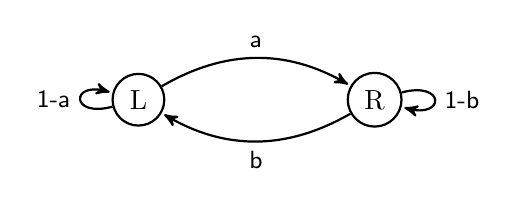
\begin{tikzpicture}[->,>=stealth',shorten >=1pt,auto,node distance=3cm,
                          thick,main node/.style={circle,draw}]
          \node[main node] (R) {R};
          \node[main node] (L) [left of=R] {L};
          \path[every node/.style={font=\sffamily\small}]
          (L) edge [loop left] node {1-a} (L)
              edge [bend left] node {a} (R)
          (R) edge [loop right] node {1-b} (R)
              edge [bend left] node {b} (L);
        \end{tikzpicture}
      \end{center}

      Then, the stationary distribution is 

        \[\boldsymbol{\pi} = \Big( \frac{b}{a+b}, \frac{a}{a+b} \Big)\]

      Notice that if $a = b = 0$, then this definition is ill-defined, and any probability distribution is invariant since $P = I_2$, the identity matrix. 
    \end{example}

    This is also stationary since with certain conditions, the limiting behavior of the chain converges to $\pi$, but we will prove that later. 

    \begin{definition}[Doubly Stochastic Chains]
      A transition matrix $\mathbf{P}$ is said to be \textbf{doubly stochastic} if its columns also sum to $1$. 
    \end{definition}

    \begin{theorem}
      Given a Markov chain with state space $S = \{1, \ldots, d\}$, its transition probability matrix $\mathbf{P}$ is doubly stochastic if and only if its stationary distribution is the uniform distribution 

        \[\boldsymbol{\pi} = \bigg( \frac{1}{d}, \frac{1}{d}, \ldots, \frac{1}{d} \bigg)\]
    \end{theorem}
    \begin{proof}
      We prove the only if part. Let $\pi(i) = 1/N$ for all $i = 1, \ldots, N$. Then, for $j = 1, \ldots, N$, 

        \[(\boldsymbol{\pi} \mathbf{P}) (i) = \sum_{j=1}^N \pi(j) \mathbf{P}(j, i) = \frac{1}{N} \sum_{j=1}^N \mathbf{P}(j, i) = \frac{1}{N} = \pi(i) \]

      The if part is very similar. 
    \end{proof}


    \subsubsection{Uniqueness}

      TBD
      TBD

    \subsubsection{Reversed Markov Process}

      From now, given the state space $(S, \mathcal{S})$ we can put a measure $\mu$ on it to get a measure space $(S, \mathcal{S}, \mu)$. The Banach space of all $\mu$-measurable functions $f: (S, \mathcal{S}, \mu) \rightarrow (\mathbb{R}, \mathcal{R})$ (i.e. for every Borel $B \in \mathcal{R}$, $f^{-1}(B) \in \mathcal{S}$) will be denoted $L^p (\mu)$, equipped with the norm 
      \[||f||_{L^p(\mu)} \coloneqq \mathbb{E}_\mu [f^p]^{1/p} = \bigg( \int_S |f|^p \,d\mu \bigg)^{1/p}\]
      If $p = 2$, then we can define the inner product 
      \[\langle f, g \rangle_\mu \coloneqq \mathbb{E}_\mu [f g] = \int_S f g \, d\mu\]

      \begin{lemma}[Contraction of Stationary Measure]
      Let $\mu$ be a stationary measure. Then, 
      \[||P_t f||_{L^p(\mu)} \geq ||f||_{L^p (\mu)} = \mathbb{E}_\mu [f^p]^{1/p}\]
      \end{lemma}

      Now, we can construct reversed Markov processes. 

      \begin{definition}[Reversed Markov Process]
      Let $\{X_n\}_{n=0}^N$ be a discrete time Markov process with transition operator $P = P_1$ (and semigroup $(P_m = P^m)$) and stationary distribution $\mu$. Then, fix $N$ and let $Y_n = X_{N - n}$. Then, $Y_n$ is a discrete time Markov process with the \textbf{dual transition operator} $P^*$, the adjoint of $P$ satisfying 
      \[\langle f, P g \rangle_\mu = \langle P^* f, g \rangle_\mu\]
      for all bounded measurable $f, g \in L^2 (\mu)$. 
      \end{definition}

      Though we have given the reversed Markov process as a definition above, we can prove that this satisfies the Markov property. 

      \begin{proof}

      \end{proof}

      We can see how this definition realizes in a discrete space. 

      \begin{example}
      Given $S = \{1, \ldots, d\}$ and function vectors $\mathbf{f}, \mathbf{g}$, 
      \[\langle f, g \rangle_\mu = \int_S f g d\mu = \sum_{i=1}^d f_i g_i \pi(i)\]
      and by definition of the adjoint, we must have 
      \begin{align*}
          \langle f, P g \rangle_\mu = \sum_{i=1}^d f_i (\mathbf{P} \mathbf{g})_i \pi(i) & = \sum_{i=1}^d f_i \bigg( \sum_{j=1}^d \mathbf{P}(i, j) g_j \bigg) \pi(i) \\
          & = \sum_{i=1}^d g_i \bigg( \sum_{j=1}^d \mathbf{P}^* (i, j) f_j \bigg) \pi(i) = \sum_{i=1}^d (\mathbf{P}^* \mathbf{f})_i \, g_i \, \pi(i) = \langle P^* f, g \rangle_\mu 
      \end{align*}
      A bit of computation will show us that 
      \[\mathbf{P}^*(i, j) = \frac{\mathbf{P}(j, i) \pi(j)}{\pi(i)}\]
      and we can indeed check that 
      \begin{align*}
          \langle P^* f, g \rangle_\mu  & = \sum_{i=1}^d g_i \bigg( \sum_{j=1}^d \mathbf{P}^* (i, j) f_j \bigg) \pi(i) \\
          & = \sum_{i=1}^d g_i \bigg( \sum_{j=1}^d f_j \frac{\mathbf{P}(j, i) \pi(j)}{\pi(i)} \bigg) \pi(i) \\
          & = \sum_{j=1}^d \sum_{i=1}^d g_i \, f_j \mathbf{P}(j, i) \, \pi(j) \\
          & = \sum_{j=1}^d f_j \bigg( \sum_{i=1}^d g_i \mathbf{P}(j, i) \bigg) \pi(j) \\
          & = \sum_{j=1}^d f_j (\mathbf{P} \mathbf{g})_j \pi(j) = \langle f, P g \rangle_\mu
      \end{align*}
      Note that $\mathbf{P}^*$ also satisfies $\mathbf{P}^* (i, j) \geq 0$ and by definition of the stationary distribution $\pi$, 
      \[\sum_{j=1}^d \mathbf{P}^* (i, j) = \sum_{j=1}^d \frac{\mathbf{P}(j, i) \pi(j)}{\pi(i)} = \frac{1}{\pi(i)} \sum_{j=1}^d \mathbf{P}(j, i) \pi(j) = \frac{\pi(i)}{\pi(i)} = 1 \]
      \end{example}

      Note that the transition probability is computed using Bayes rule 
      \begin{align*}
          \mathbf{P^*}(i, j) & = \mathbb{P}(Y_{m + 1} = j \mid Y_m = i) \\
          & = \frac{\mathbb{P}(Y_m = i \mid Y_{m+1} = j) \mathbb{P}(Y_{m+1} = j)}{\mathbb{P}(Y_m = i)} \\
          & = \frac{\mathbb{P}(X_{n-m} = i \mid X_{n-m-1} = j) \mathbb{P}(X_{n-m-1} = j)}{\mathbb{P}(X_{n-m} = i)} \\
          & = \frac{\mathbf{P}(j, i) \pi(j)}{\pi(i)}
      \end{align*}
      and $\{Y_m\}$ also satisfies the Markov property. 
      \begin{align*}
          \mathbb{P}&(Y_{m+1} = j \mid Y_m = i, Y_{m-1} = i_{m-1}, \ldots, Y_0 = i_0) \\
          & = \frac{\mathbb{P}(Y_0 = i_0, \ldots, Y_{m-1} = i_{m-1}, Y_{m} = i, Y_{m+1} = j)}{\mathbb{P}(Y_0 = i_0, \ldots, Y_{m-1} = i_{m-1}, Y_{m} = i)} \\
          & = \frac{\mathbb{P}(X_n = i_0, \ldots, X_{m-n+1} = i_{m-1}, X_{n-m} = i, X_{n-m-1} = j)}{\mathbb{P}(X_n = i_0, \ldots, X_{m-n+1} = i_{m-1}, X_{n-m} = i)} \\
          & = \frac{\mathbb{P}(X_n = i_0, . , X_{m-n+1} = i_{m-1} \mid X_{n-m} = i, X_{n-m-1} = j) \mathbb{P}(X_{n-m} = i \mid X_{n-m-1} = j) \mathbb{P}(X_{n-m-1} = j)}{\mathbb{P}(X_n = i_0, \ldots, X_{m-n+1} = i_{m-1} \mid X_{n-m} = i) \mathbb{P}(X_{n-m} = i)} \\
          & = \frac{\mathbb{P}(X_n = i_0, \ldots, X_{m-n+1} = i_{m-1} \mid X_{n-m} = i) p(j, i) \pi(j)}{\mathbb{P}(X_n = i_0, \ldots, X_{m-n+1} = i_{m-1} \mid X_{n-m} = i) p(i)} \\
          & = \frac{p(j, i) \pi(j)}{p(i)}
      \end{align*}
      Thus, $\{Y_m\}$ is a Markov chain with the indicated transition probability. 

  \subsection{Reversibility (Detailed Balance)}

    Note that reversibility of a Markov process and a reversed Markov process are two entirely different things. There is always a reveresed Markov process, but the fact that it is reversible is a much stronger condition. 

    \begin{definition}[Reversibility]
      The Markov semigroup $\{P_m\}$ with stationary measure $\mu$ is called \textbf{reversible} (or in the physics literature, is said to satisfy \textbf{detailed balance}) if $P_m$ is self-adjoint for every $f, g, \in L^2 (\mu)$. That is, 

        \[\langle f, P_m g \rangle_\mu = \langle P_m f, g \rangle_\mu\]

      By the properties of the adjoint and the Chapman-Kolmogorov equation, we only need to check if $P$ is adjoint. 
    \end{definition}

    Note that if the Markov property is reversible, then assuming $X_0 \sim \mu$, then 

    \begin{align*}
      \langle P_m f, g \rangle_\mu & = \langle f, P_m g \rangle_\mu = \mathbb{E}[ f(X_n) \, \mathbb{E}[g(X_{n + m}) \mid X_n]] \\
      & = \mathbb{E}[ f(X_n) \, g(X_{n + m})] = \mathbb{E}[ \mathbb{E}[ f(X_n) \mid X_{n + m})] \, g(X_{n + m}] 
    \end{align*}

    for every $f, g \in L^2 (\mu)$. So that in particular, 

      \[P_m f (x) = \mathbb{E}[f(X_{n + m} \mid X_n = x] = \mathbb{E}[f(X_n) \mid X_{n + m} = x]\]

    \begin{example}[Detailed Balance in Finite State Space]
      We know that if $P$ is self adjoint, then its transition probability matrix will satisfy 

        \[\mathbf{P}(i, j) = \frac{\mathbf{P}(j, i) \, \pi(j)}{\pi(i)} \implies \mathbf{P}(j, i) \, \pi(j) = \mathbf{P}(i, j) \, \pi(i)\]

      which is the familiar detailed balance condition that we are used to. To see that this is a stronger condition than $\mathbf{P} \boldsymbol{\pi} = \boldsymbol{\pi}$, we sum over $j$ on each side to get 

        \[\sum_j \mathbf{P}(i, j) \, \pi(i) = \pi(i) \, \sum_j \mathbf{P}(i, j) = \pi(j)\]

      Remember that we could interpret $\pi(i)$ as the amount of water at $x$, and we send $\mathbf{P}(j, i) \pi(i)$ water from node $i$ to $j$ in one step. The detailed balance condition tells us that the amount of sand going from $i$ to $j$ in one step is exactly balanced by the amount going back from $j$ to $i$. In contrast, the condition $\boldsymbol{\pi} \mathbf{P} = \boldsymbol{\pi}$ says that after all the transfers are made, the amount of water that ends up at each node is the same as the amount there. 
    \end{example}

    Many chains do not have stationary distributions that satisfy the detailed balance condition. 

    \begin{example}
      Consider the chain with 

        \[\mathbf{P} = \begin{pmatrix} .5 & .5 & 0 \\ .3 & .1 & .6 \\ .2 & .4 & .4 \end{pmatrix}\]

      There is no stationary distribution with detailed balance since $\pi(1) \pi(1, 3) = 0$ but $\mathbf{P}(1, 3) > 0$ so we must have $\pi(3) = 0$. But this would imply that $\pi(3) \mathbf{P}(3, i) = \pi(i) \mathbf{P}(i, 3)$ for all $i$ so we conclude all $\pi(i) = 0$, which doesn't make sense. In fact, the stationary distribution is $(1/3, 1/3, 1/3)$ since $\mathbf{P}$ is doubly stochastic. 
    \end{example}

    \subsubsection{Metropolis-Hastings Algorithm}

      A huge application of Markov chains are in monte carlo algorithms, specifically the Metropolis-Hastings. We begin with a Markov chain with transition probability $q(x, y)$ that is the proposed jump distribution. A move is accepted with probability 

        \[r(x, y) = \min\bigg\{ \frac{\pi(y) q(y, x)}{\pi(x) q(x, y)}, 1 \bigg\}\]

      so the transition probability becomes 

        \[p(x, y) = q(x, y) r(x, y)\]

      Why do we do this? Multiplying by $r$ guarantees that $\pi$ now satisfies detailed balance under $p$. Without loss of generality, we can assume $\pi(y) q(y, x) > \pi(x) q(x, y)$, and so we have 

      \begin{align*}
        \pi(x) p(x, y) & = \pi(x) q(x, y) \,1 \\
        \pi(y) p(y, x) & = \pi(y) q(y, x) \frac{\pi(x) q(x, y)}{\pi(y) q(y, x)} = \pi(x) q(x, y)
      \end{align*}

      which satisfies detailed balance. 

    \subsubsection{Kolmogorov Cycle Condition}

      Let us take a motivating example. 

      \begin{example}
        Consider the chain with transition probability 

          \[p = \begin{pmatrix} 1 - (a + d) & a & d \\ e & 1 - (b + e) & b \\ c & f & 1 - (c + f) \end{pmatrix}\]

        and suppose that all entries are positive. To satisfy detailed balance, we must have $\pi(x) p(x, y) = \pi(y) p(y, x)$ for all $x, y$. So we must have

          \[e \pi(2) = a \pi(1) \;\;\;\;\; f \pi(3) = b \pi(2) \;\;\;\;\; d \pi(1) = c \pi(3)\]

        Multiplying the three equations gives $abc = def$, or in other words, 

          \[\frac{p(1, 2) \, p(2, 3) \, p(3, 1)}{p(2, 1)\, p(3, 2) \, p(1, 3)} = \frac{abc}{def} = 1\]
      \end{example}

      \begin{definition}[Kolmogorov Cycle Condition]
        Given a finite irreducible Markov chain with state space $S$. We say that the \textbf{cycle condition} is satisfied if given a cycle of states $x_0, x_1, \ldots, x_n = x_0$ with $p(x_{i-1}, x_i) > 0$ for $1 \leq i \leq n$, we have 

          \[\prod_{i=1}^n p(x_{i-1}, x_i) = \prod_{i=1}^n p(x_i, x_{i-1})\]
      \end{definition}

      \begin{theorem}
        Given a Markov chain $S$ with transition probability $p$, there exists a stationary distribution $\pi$ that satisfies detailed balance if and only if the cycle condition holds. 
      \end{theorem}

  \subsection{Ergodicity}

    Now, we want to talk about "well-behaved" Markov processes that have a limiting distribution that is the stationary measure, i.e. the process will eventually end up in its steady state $\rho_n \rightarrow \mu$ as $n \rightarrow +\infty$ even if it is not started there. That is, given some fixed initial condition $X_0 = x$, is it true that 

      \[\mathbb{E}[f(X_n) \mid X_0 = x] \rightarrow \mathbb{E}_\mu [f] \text{ as } n \rightarrow \infty\]

    \begin{definition}[Ergodicity]
      The Markov semigroup $(P_n)$ is called \textbf{ergodic} if 

        \[P_n f \rightarrow \mu(f) = \mathbb{E}_\mu [f]\]

      as $n \rightarrow +\infty$ for every $f \in L^2 (\mu)$ (i.e. converges to the constant function $\mu f = \mu(f)$). That is, if we would like to measure $X_n \sim \rho_n$ with $f$, then far enough in time this measurement converges to measuring $X \sim \mu$ with $f$. Since this applies to all $f$ (think $f = 1_A$), we can determine that $\rho_n \rightarrow \mu$ as $n \rightarrow +\infty$. 
    \end{definition}

    The following theorem determines whether a chain is ergodic, but note that we don't know anything about the \textit{rate of convergence} to the stationary measure. 

    \begin{theorem}
      If Markov process $\{X_n\}$ with stationary measure $\mu$ and semigroup $(P_n)$ is irreducible, then $(P_n)$ is ergodic. 
    \end{theorem}

    \begin{theorem}
      Suppose $|S| < \infty$. If the chain is irreducible and all states positive recurrnent, then there always exists a unique stationary distribution $\pi$. If the chain is also aperiodic, then for any initial distribution $\nu$, 

        \[\lim_{k \rightarrow \infty} \nu P^k = \pi \]

      Hence

        \[\lim_{k \rightarrow \infty} P^{(k)}(x, y) = \pi(y)\]

      for all $x, y \in S$. Furthermore, for any measurable function $f: S \longrightarrow \mathbb{R}$, the limit 

        \[\lim_{N \rightarrow \infty} \frac{1}{N} \sum_{n=1}^N f(X_n) = \sum_{x \in S} f(x)\, \pi(x) = \mathbb{E} \big( f(x) \big)\]

      holds with probability $1$. In particular, the limit does not depend on the initial distribution. 
    \end{theorem}
    \begin{proof}
      The Frobenius Extension to Perron's theorem (Linear Algebra, Theorem 7.31) combined with its applications to stochastic matrices (Linear Algebra, Theorem 7.30) proves this statement. 
    \end{proof}

    The next result describes the limiting fraction of time we spend in each state. 

    \begin{theorem}[Asymptotic Frequency]
      Suppose we have a finite Markov chain with $p$ irreducible and all states recurrent. Then, let 

        \[N_n (y) = \sum_{i=1}^n 1_{X_i = y}\]

      be the number of visits to $y$ up to time $n$. Then, 

        \[\frac{N_n (y)}{n} \rightarrow \frac{1}{\mathbb{E}_y [T_y]}\]

      If the chain is aperiodic, then we also have 

        \[\pi(y) = \frac{1}{\mathbb{E}_y [T_y]}\]
    \end{theorem}

    \begin{theorem}
      Suppose that a chain is irreducible and there exists stationary distribution $\pi$. Then, 

        \[\frac{1}{n} \sum_{m=1}^n p^m (x, y) \rightarrow \pi(y)\]

      Thus while the sequence $p^m (x, y)$ will not converge in the periodic case, the average of the first $n$ values will. 
    \end{theorem}

\section{Poisson Processes}

  \subsection{Exponential Distribution}

    Let us do some review. The \textbf{exponential distirbution} of rate $\lambda$ is a random variable $T \sim \mathrm{Exponential}(\lambda)$ with CDF 

      \[F_T (t) = \mathbb{P}(T \leq t) = 1 - e^{-\lambda t}\]

    and the PDF 

      \[f_T (t) = \begin{cases} \lambda e^{-\lambda t} & t \geq 0 \\ 0 & t < 0 \end{cases}\]

    We have 

      \[\mathbb{E}[T] = \frac{1}{\lambda}, \;\; \mathrm{Var}(T) = \frac{1}{\lambda^2}\]

    \begin{lemma}[Memoryless Property]
      The Exp$(\lambda)$ distribution has the property that for all $t, s \geq 0$, 

        \[\mathbb{P}(W > t + s \; | \; W > t) = \mathbb{P}(W > s)\]

      which is called the \textit{memoryless property}. We can interpret this in the following way. Let $W$ be the time you have to wait for the first arrival. Given that you already waited $t$ units of time, the probability that you have the wait $s$ additional units of time is just the probability that you wait at least $s$ from the beginning. That is, knowing that $t$ units of time have elapsed does not affect the distribution of the remaining waiting time. 
    \end{lemma}

    \begin{theorem}
      Let $W$ be a continuously distributed random variable. Then $W \sim$ Exp$(\lambda)$ for some $\lambda > 0$ if and only if $W$ satisfies the memoryless property. 
    \end{theorem}

    \begin{theorem}
      Let $T_i \sim \mathrm{Exponential}(\lambda_i)$ for $i = 1, \ldots n$. Then, 

        \[\min\{T_1, \ldots, T_n\} \sim \mathrm{Exponential}(\lambda_1 + \ldots + \lambda_n)\]

      and the random variable $I$ which takes the index of $\min\{T_1, \ldots, T_n\}$ has the PMF 

        \[\mathbb{P}(I = i) = \frac{\lambda_i}{\lambda_1 + \ldots + \lambda_n}\]
    \end{theorem}

  \subsection{Defining the Poisson Process}

    We first describe a limiting behavior of binomial random variables. 

    \begin{theorem}[Poisson Limit Theorem]
      Let $X_n \sim \mathrm{Bernoulli}(n, p_n)$, where $\{p_n\}_{n \in \mathbb{N}}$ is a sequence of reals in $[0, 1]$ such that 

        \[\lim_{n \rightarrow \infty} n p_n = \lambda\]

      Letting $Y \sim \mathrm{Poisson}(\lambda)$

        \[X_n \xrightarrow{D} Y\]

      That is, the CDFs, and since this is a discrete distribution, the PMFs, converge. 
    \end{theorem}
    \begin{proof}
      We will show that $\lim_{n \rightarrow \infty} \mathbb{P}(X_n = k) = \mathbb{P}(Y = k)$, which shows that the CDFs converge and therefore convergence in distribution. 
      \begin{align*}
        \lim_{n \rightarrow \infty} \mathbb{P}(X_n = k) & = \lim_{n \rightarrow \infty} \binom{n}{k} p_n^k (1 - p_n)^k \\
        & = \lim_{n \rightarrow \infty} \frac{n (n - 1) \ldots (n - k + 1)}{k!} \bigg(\frac{\lambda}{n}\bigg)^k \bigg( 1 - \frac{\lambda}{n} \bigg)^{n - k} \\
        & = \lim_{n \rightarrow \infty} \frac{n^k + O(n^{k-1})}{k!} \frac{\lambda^k}{n^k} \bigg( 1 - \frac{\lambda}{n} \bigg)^{n - k} \\
        & = \lim_{n \rightarrow \infty} \frac{\lambda^k}{k!} \bigg( 1 - \frac{\lambda}{n} \bigg)^{n - k} \\
        & = \frac{\lambda^k}{k!} \lim_{n \rightarrow \infty} \bigg( 1 - \frac{\lambda}{n} \bigg)^n \; \lim_{n \rightarrow \infty} \bigg( 1 - \frac{\lambda}{n} \bigg)^{-k} \\
        & = \frac{\lambda^k}{k!} \, e^{\lambda} \, 1 = \frac{\lambda^k e^\lambda}{k!}
      \end{align*}
    \end{proof}

    Note that this is different from CLT because in CLT, we just assume that the $p_n$'s are constant and take the limiting behavior of $X_n \sim \mathrm{Bernoulli}(n, p)$ as $n \rightarrow \infty$. 

    This result justifies the following model. A Poisson Arrival Process with rate $\lambda > 0$ on the interval $[0, \infty)$ is a model for the occurrence of some events which may have at any time. We can interpret the process as a collection of random points in $[0, \infty)$ which are the times at which the arrivals occur. Suppose that we would like to model the arrival of events that happen completely at random at a rate $\lambda$ per unit time. At time $t = 0$, we have no arrivals yet, so $N(0) = 0$. Let us fix some $T$, and now divide $[0, T)$ into $n$ tiny subintervals of length $\delta$. 

    \begin{center}
      %\includegraphics[scale=0.3]{}
    \end{center}

    Assume that in each time slot, we assign a $X_k \sim \mathrm{Bernoulli}(\lambda \delta)$ random variable that determines whether there was an arrival within the interval $((k-1)\delta, k\delta]$. So with probability $\lambda\delta$, there will be an arrival within it, and as the time interval gets smaller, this probability also gets smaller too. Since every $n$ subinterval is $\mathrm{Bernoulli}(\lambda \delta)$, the number of arrivals in the interval $[0, T)$, defined as the random variable $N_n (T)$, is 

      \[N_n (T) \sim \mathrm{Binomial}(n, \lambda \delta) = \mathrm{Binomial}\big(n, \frac{\lambda T}{n}\big)\]

    As we increase the $n$ (equivalently, decrease $\delta$), we divide $[0, T)$ into smaller and smaller subintervals, resulting in finer and finer $N_n(T)$ Binomial distributions. Since $n p_n = n \frac{\lambda T}{n} = \lambda T$ is finite, we can invoke the Poisson limit theorem and say 

      \[N_n (T) \xrightarrow{D} \mathrm{Poisson}(\lambda T)\]

    Note that the starting point $0$ does not matter, and this works for any interval of length $T$. Therefore, we can model the arrival times on any interval of length $T$ as a $\mathrm{Poisson}(\lambda T)$ random variable. 

    \begin{definition}[Poisson Process]
      Let $\lambda > 0$ be fixed, representing the rate of arrival in some unit time. The stochastic counting process $\{N(t)\}_{t \geq 0}$, where $N(t)$ represents the number of arrivals by time $t$, is called a \textbf{Poisson process} with rate $\lambda$ if 
      \begin{enumerate}
        \item $N(0) = 0$ 

        \item The number of arrivals in any interval of length $s > 0$ is $N(t + s) - N(t) \sim \mathrm{Poisson}(\lambda s)$ 

        \item $N(Tt)$ has independent increments, i.e. if $t_0 < t_1 < \ldots, < t_n$, then 

          \[N(t_1) - N(t_0), \ldots, N(t_n) - N(t_{n-1})\]

        are independent. 
      \end{enumerate}
    \end{definition}

  \subsection{Constructing the Poisson Process}

    Now we have modeled this process using random variables $N(t)$ that counts the number of arrivals up to time $t$. Now, we can interpret it using random variables that represent the \textit{time} in which they arrive. 

    \begin{definition}
      Set $T_0 = 0$. The arrival times are random variables $0 < T_1 < T_2 < T_3 < \ldots$ such that the inter-arrival waiting times

        \[\tau_k = T_k - T_{k-1}, \;\;\; k \geq 0\]

      have the property that $\{W_k\}_{k=1}^\infty$ are independent $\mathrm{Exp}(\lambda)$ random variables. Define 

        \[N(s) \coloneqq \max\{k \mid T_k \leq s \}\]
    \end{definition}

    Now we prove that this process is equivalent to the Poisson process defined before. 

    \begin{theorem}[Equivalent Interpretations]
      Let $\{T_n\}$ be defined as above and $N(s) \coloneqq \max\{k \mid T_k \leq s \}$. Then, 

      \begin{enumerate}
        \item $N(0) = 0$
        \item $N(s) \sim \mathrm{Poisson}(\lambda s)$ 
        \item $N(t + s) - N(t) \sim \mathrm{Poisson}(\lambda s)$ independent of $N(r)$ for $0 \leq r \leq s$. 
        \item $N(t)$ has independent incremements. 
      \end{enumerate}

      $N(s) \coloneqq \max\{k \mid T_k \leq s \}$ is a Poisson distribution with mean $\lambda s$. 
    \end{theorem}

\section{Continuous-Time Markov Processes}

  As the name suggests, in a continuous time Markov process $X_t$, the time parameter is continuous ($t \geq 0$). As before, the system jumps randomly between states in $S$, but now the jumps may occur at any time and they occur randomly. This implies that there are \textit{two} sources of randomness:

  \begin{enumerate}
    \item \textit{where} the system jumps, which is determined by the transition probabilities, and 
    \item \textit{when} the system jumps, which is called the holding time
  \end{enumerate}

  \begin{definition}[CTMP]
    Let $(\Omega, \mathcal{F}, \mathbb{P})$ be a probability space and $(S, \mathcal{S})$ a measurable space. Then, a homogeneous \textbf{continuous-time Markov chain} is a stochastic process $\{X_t\}_{t \geq 0}$ taking values in $S$ (i.e. $X_t: \Omega \rightarrow S$) satisfying the \textbf{Markov property}: for every bounded measurable $f$ and and $t, s \geq 0$, 

      \[\mathbb{E}[ f(X_{t + s}) \mid \{X_r\}_{r \leq t} ] = \mathbb{E}[ f(X_{t + s}) \mid X_t ] = (P_s f)(X_t)\]

    This again says that the probability of $X_{t + s}$ does not depend on the history $\{X_r = i_r\}_{r \leq t}$, but on the current value of $X_t$. 
  \end{definition}

  Just like the discrete-time case, to describe random variable $X_{t + s}$ with function $f$, we can pull back the function to compute 

    \[\mathbb{E}[f(X_{t + s})] = \mathbb{E}[ \mathbb{E}[ f(X_{t + s}) \mid X_t]] = \mathbb{E}[ (P_s f) (X_t)] = \int_S P_s f \, d\rho_t\]

  which integrates a new function $P_s f$ over the measure $\rho_t$. 

  \begin{example}[Transition Operator as a Matrix in Discrete Space]
    Let us have a discrete space $S = \{1, \ldots, d\}$ with indicators $1_{\{i\}}$ for $i = 1, \ldots, d$. Let $x_t$ represent the column vector of the PMF of $X_t$. From the same work as shown for discrete time Markov processes, we can let $f = 1_{\{j\}}$ and compute the probability of $X_{t + s}$ landing in each point $j \in S$, since that is what we're interested in for discrete probability distributions. 

    \begin{align*}
      \boldsymbol{\rho_{t + s}} (j) & = \mathbb{P}( X_{t + s} = j) \\ 
      & = \mathbb{E}[1_{\{j\}} (X_{t + s})] \\
      & = \mathbb{E} [ \mathbb{E}[ 1_{\{j\}} (X_{t + s}) \mid X_t] ] && = \mathbb{E}[P_s 1_{\{j\}} (X_t)] \\
      & = \int_S \mathbb{E}[ 1_{\{j\}} (X_{t + s}) \mid X_t] d\rho_t && = \int_S P_s 1_{\{j\}} (X_t) \,d \rho_t \\
      & = \sum_{i \in S} \mathbb{P}[ X_{t + s} = j \mid X_t = i] \, \mathbb{P} ( X_t = i) && = \sum_{i \in S} P_s 1_{\{j\}} (i) \mathbb{P}(X_t = i) 
    \end{align*}

    which can be summarized as 

      \[\boldsymbol{\rho_{t + s}} (j) = \sum_{i = 1}^d P_s 1_{\{j\}} (i) \boldsymbol{\rho_t} (i) = \sum_{i = 1}^d \mathbb{P}(X_{t + s} = j \mid X_t = i) \, \boldsymbol{\rho_t} (i)\]

    We can compactly organize the probabilities of these internode travel inside a $d \times d$ right stochastic \textbf{transition matrix}

      \[\mathbf{P_s} = \begin{pmatrix} P_s 1_{\{1\}} (1) & \ldots & P_s 1_{\{1\}} (d) \\ \vdots & \ddots & \vdots \\ P_s 1_{\{d\}} (1) & \ldots & P_s 1_{\{d\}} (d) \end{pmatrix} = \begin{pmatrix} \mathbb{P}(X_{t + s} = 1 \mid X_t = 1) & \ldots & \mathbb{P}(X_{t + s} = d \mid X_t = 1) \\ \vdots & \ddots & \vdots \\ \mathbb{P}(X_{t + s} = 1 \mid X_t = d) & \ldots & \mathbb{P}(X_{t + s} = d \mid X_t = d) \end{pmatrix} \]

    and compactly write the above equation as 

      \[\boldsymbol{\rho_{t + s}}^T = \boldsymbol{\rho_{t}}^T \mathbf{P_s}\]
  \end{example}

  \begin{lemma}
    $P_t$ is linear. That is, for $t, s \geq 1$, $\alpha, \beta \in \mathbb{R}$, and bounded measurable functions $f, g$, 

      \[P_t (\alpha f + \beta g) = \alpha P_t f + \beta P_t g\] 
  \end{lemma}
  \begin{proof}
    By linearity of conditional expectation, 
    \begin{align*}
      (P_s (\alpha f + \beta g))(X_t) & = \mathbb{E}[(\alpha f + \beta g)(X_{t + s}) \mid X_t] \\
      & = \mathbb{E}[(\alpha f) (X_{t + s}) \mid X_t] + \mathbb{E}[(\beta g) (X_{t + s}) \mid X_t] \\
      & = \alpha (P_s f) (X_t) + \beta (P_s g) (X_t)
    \end{align*}
  \end{proof}

  We can now interpret linearity and the Markov property in the discrete space. 

  \begin{example}[Markov Property in Discrete Space]
    If we wanted to extract information from $X_t$ with function $f$ (i.e. compute $\mathbb{E}[f(X_t)]$), we can calculate 

      \[\mathbb{E}[f(X_t)] = \boldsymbol{\rho_t}^T \mathbf{f} =  \begin{pmatrix} \boldsymbol{\rho_t} (1) & \ldots & \boldsymbol{\rho_t} (d) \end{pmatrix} \begin{pmatrix} f_1 \\ \vdots \\ f_d \end{pmatrix}\] 

    Now, say that $s$ units of time later, we want to extract information $f$ from $X_{t + s}$ by computing 

      \[\mathbb{E}[f(X_{t + s})] = \boldsymbol{\rho_{t + s}}^T \mathbf{f} = \begin{pmatrix} \boldsymbol{\rho_{t + s}} (1) & \ldots &  \boldsymbol{\rho_{t + s}} (d) \end{pmatrix} \begin{pmatrix} f_1 \\ \vdots \\ f_d \end{pmatrix}\]

    The problem is that we don't know what the distribution of $X_{t + s}$ is (i.e. don't know $\boldsymbol{\rho_{t + s}} (i)$), so we get its expectation by conditioning it on $X_t$, which realizes as taking the expectation of a \textit{different} function $P_s f$ with respect to $\rho_t$. 

      \[\mathbb{E}[f(X_{t + s})] = \mathbb{E}[ \mathbb{E}[ f(X_{t + s}) \mid X_t]] = \mathbb{E}[(P_s f)(X_t)] = \begin{pmatrix} \boldsymbol{\rho_t} (1) & \ldots & \boldsymbol{\rho_t} (d) \end{pmatrix} \begin{pmatrix} (P_s f)_1 \\ \vdots \\(P_s f)_d \end{pmatrix}\]

    It turns out that this transformation $\mathbf{f} \mapsto \mathbf{P_s} \mathbf{f}$ (from row vector to row vector) is linear, and so we can interpret $\mathbf{P_s}$ as $\mathbf{f}$ that has been left-multiplied by some transformation matrix $\mathbf{P_s}$. 

      \[\begin{pmatrix} \boldsymbol{\rho_t} (1) & \ldots & \boldsymbol{\rho_t} (d) \end{pmatrix} \begin{pmatrix} (P_s f)_1 \\ \vdots \\(P_s f)_d \end{pmatrix} = \begin{pmatrix} \boldsymbol{\rho_t} (1) & \ldots & \boldsymbol{\rho_t} (d) \end{pmatrix} \underbrace{\begin{pmatrix} && \\ & \mathbf{P_s} & \\ && \end{pmatrix} \begin{pmatrix} f_1 \\ \vdots \\ f_d \end{pmatrix}}_{\mathbf{P_s f}}\]

    It turns out that this $\mathbf{P_s}$ acts linearly on $\mathbf{f}$ through left multiplication, but we can also right-multiply $\boldsymbol{\rho_t}$ by $\mathbf{P_s}$ to get the new distribution of $X_{t + s}$! 

      \[\begin{pmatrix} \boldsymbol{\rho_t} (1) & \ldots & \boldsymbol{\rho_t} (d) \end{pmatrix} \begin{pmatrix} (P_s f)_1 \\ \vdots \\(P_s f)_d \end{pmatrix} = \underbrace{\begin{pmatrix} \boldsymbol{\rho_t} (1) & \ldots & \boldsymbol{\rho_t} (d) \end{pmatrix} \begin{pmatrix} && \\ & \mathbf{P_s} & \\ && \end{pmatrix}}_{\boldsymbol{\rho_t}^T \mathbf{P_s} = \boldsymbol{\rho_{t+s}}^T} \begin{pmatrix} f_1 \\ \vdots \\ f_d \end{pmatrix}\]

    Therefore, it turns out that the linearity of $\mathbf{P_s}$ on $\mathbf{f}$ implies linearity of it on the vector $\boldsymbol{\rho_t}$. 
  \end{example}

  Now focusing on $f = 1_A$, we can define the following. 

  \begin{definition}[Transition Probability]
  Let us have Markov process $(X_t)$ with operator $P_s$. The function $p_s: S \times \mathcal{S} \rightarrow \mathbb{R}$ defined 

    \[p_s(x, A) \coloneqq P_s 1_A (x) = \mathbb{E}[ 1_A (X_{t+s}) \mid X_t = x] = \mathbb{P}(X_{t + s} \in A \mid X_t = x)\]

  is the \textbf{transition probability}, or \textbf{transition kernel}, of this chain. Note that 

  \begin{enumerate}
    \item For each $x \in S$, $A \mapsto p_s(x, A)$ is a probability measure on $(S, \mathcal{S})$. This means that if we are in some place $x$ at time $t$, then the probability that we will land in some subset $A \in \mathcal{S}$ of $S$ at time $t + s$ is $p_s(x, A)$. 
    \item For each $A \in \mathcal{S}$, $P_s 1_A = p_s (\cdot, A)$ is a measurable function. 
  \end{enumerate}
  The \textbf{transition kernel density} is simply the pdf of the measure $p_s(x, \cdot)$. 

    \[p_s(x, A) = \int_A p_s (x, y) \,dy\]
  \end{definition}

  Note that in the matrix realization of the example above, it looks like $P_s$ acts on the distribution $\rho_t$ to get a new distribution $\rho_{t + s}$, but this is not strictly the case since $P_s$ is an operator on $f$. However, for the sake of intuitiveness, we can interpret $P_s$ in two ways: 

  \begin{enumerate}
    \item It operates on the measure $\rho_t$ by pushing it forward in time to get $\rho_{t + s}$. This operator is defined as 

      \[\rho_t \mapsto \rho_{t + s}(\cdot) = p_s (X_t, \cdot)\]

    which corresponds to the matrix multiplication $\boldsymbol{\rho_t}^T \mapsto \boldsymbol{\rho_{t + s}}^T = \boldsymbol{\rho_{t}}^T \mathbf{P_s}$

    \item It operates on the function $f$ (at $X_{t + s}$) by pulling it back to $P_s f$ that operates on $X_t$. This operation $f \mapsto P_s f$ corresponds to the matrix multiplication $\mathbf{f} \mapsto \mathbf{P_s} \mathbf{f}$. 

  \end{enumerate}

  Either way, we can think of the order of operations as either $(\boldsymbol{\rho_t}^T \mathbf{P_s}) \mathbf{f}$ or $\boldsymbol{\rho_t}^T (\mathbf{P_s} \mathbf{f})$. 

  Just like stochastic transition matrices, we can also deduce a semigroup property of the collection $(P_s)_{s \geq 0}$. 

  \begin{lemma}[Chapman-Kolmogorov]
  $\{P_t\}$ satisfies 
  \[P_{t + s} f = P_t P_s f\]
  for all $t, s, \geq 1$, with $P_0 = I$, the identity. 
  \end{lemma}
  \begin{proof}
  We can easily see that $(P_0 f) (X_t) = \mathbb{E}[f(X_t) \mid X_t] = f(X_t)$, and 
  \begin{align*}
      (P_{t + s} f) (X_n) & = \mathbb{E}[ f(X_{n + t + s}) \mid X_n] \\
      & = \mathbb{E} [ \mathbb{E}[ f(X_{n + t + s} \mid X_{n + t}) ] \mid X_n] \\
      & = \mathbb{E}[(P_s f) (X_{n + t}) \mid X_n] \\
      & = (P_t (P_s f))(X_n) \\
      & = (P_t P_s f) (X_n)
  \end{align*}
  \end{proof}

  We give one final condition. 

  \begin{lemma}[Conservativeness]
  $\{P_t\}$ satisfies 
  \[P_t 1 = 1\]
  for all $t \geq 0$, where $1 = 1_S$ is the constant function of $1$. 
  \end{lemma}
  \begin{proof}
  This is trivial since it is just the law of total probability. That is, $1_S (X_t) = 1$, and 
  \[(P_s 1_S) (X_t) = \mathbb{E}[ 1_S (X_{t + s}) \mid X_t]\]
  and note that $\sigma(X_t)$ is a finer $\sigma$-algebra than that generated by $1_S (X_{t + s})$, meaning that the right hand side is equal to $1_S (X_{t + s})$ itself, which equals $1$. 
  \end{proof}

  \begin{example}
  Given the transition matrix 
  \[\mathbf{P_s} = \begin{pmatrix} P_s 1_{\{1\}} (1) & \ldots & P_s 1_{\{1\}} (d) \\ \vdots & \ddots & \vdots \\ P_s 1_{\{d\}} (1) & \ldots & P_s 1_{\{d\}} (d) \end{pmatrix}\]
  note that by linearity of $P_s$ and the fact that $\{j\}$ forms a partition of $S$, we have a
  \[\sum_{j \in S} (P_s 1_{\{j\}}) (i) = \bigg[ P_s \bigg( \sum_{j \in S} 1_{\{j\}} \bigg) \bigg] \big( i \big) = (P_s 1_S) (i) = 1_S (i) = 1\]
  which means that the columns must sum to $1$. 
  \end{example}

  \begin{example}[Markov Chain with Continuous Jumps]
  Let $N(t), t \geq 0$ be a Poisson process with rate $\lambda$ and let $Y_n$ be a discrete time Markov chain with transition probability $u(i, j)$. Then, $X_t = Y_{N(t)}$ is a continuous time Markov chain that takes one jump according to $u(i, j)$ at each arrival time $N(t)$. 
  \end{example}


  \subsection{Generator}

    In the discrete time case, we had $P_t = (p_1)^t$ for $t \in \mathbb{N}$, and from the Chapman-Kolmogorov equation, knowing $p_1$ allows us to compute $p_t$ for all $t \in \mathbb{N}$. Likewise, if we know the transition probability for some $t < t_0$ for any $t_0 > 0$, we know it for all $t$. This observation suggests that the transition probabilities $p_t$ can be determined from their derivatives at $0$. 

    We now define the analogous operator to the transition rate matrix in continuous-time chains with a finite state space. This is a natural extension, since we are just taking the right-derivative of $P_t$ at $t = 0$. 

    \begin{definition}[Generator]
    The generator $\mathscr{L}$ is defined as 
    \[\mathscr{L} f \coloneqq \lim_{t \downarrow 0} \frac{P_t f - f}{t}\]
    for every $f \in L^2 (\mu)$ for which the above limit exists in $L^2 (\mu)$. Intuitively, $\mathscr{L} f$ represents the instantaneous rate of change of the measurement $f$. The set of $f$ for which $\mathscr{L}f$ is defined is called the domain $\mathrm{Dom}(\mathscr{L})$ of the generator, and $\mathscr{L}$ defines a linear operator from $\mathrm{Dom}(\mathscr{L}) \subset L^2 (\mu)$ to $L^2 (\mu)$. 
    \end{definition}

    We have defined the generator $\mathscr{L}$ from the Markov semigroup $\{P_t\}_{t \geq 0}$. Now, let's try to define the semigroup in terms of the generator $\mathscr{L}$. Given that we have some map $\mathscr{L})$, can we define some semigroup $\{P_t\}$ satisfying the definition? We know that by the semigroup property, we can split $P_{t + h}$ into $P_t P_h$ and $P_h P_t$, from which we get the \textbf{Kolmogorov backward equation} and the \textbf{forward equation}, respectively. 
    \begin{align*}
        \frac{d}{dt} P_t & = \lim_{h \downarrow 0} \frac{P_{t + h} - P_t}{h} = \lim_{h \downarrow 0} \frac{P_t ( P_h - I)}{h} = P_t \bigg( \lim_{h \downarrow 0} \frac{P_h - I}{h} \bigg) = P_t \mathscr{L} \\
        \frac{d}{dt} P_t & = \lim_{h \downarrow 0} \frac{P_{t + h} - P_t}{h} = \lim_{h \downarrow 0} \frac{( P_h - I) P_t}{h} = \bigg( \lim_{h \downarrow 0} \frac{P_h - I}{h} \bigg) P_t = \mathscr{L} P_t
    \end{align*}
    From which we see that the generator $\mathscr{L}$ is commutes with the semigroup 
    \[\mathscr{L} P_t = P_t \mathscr{L}\]
    and solving this differential equation gives 
    \[P_t = e^{t \mathscr{L}}\]

    Let's observe how this generator acts on the indicator functions $f = 1_A$. Note that $P_s 1_A (i) = \mathbb{P}(X_{t + s} \in A \mid X_t = i)$. 
    \[(\mathscr{L} 1_A) (i) = \bigg( \lim_{h \downarrow 0} \frac{P_h 1_A - 1_A}{h} \bigg) (i) = \lim_{h \downarrow 0} \frac{ P_h 1_A (i) - 1_A (i)}{h}\]
    and so $(\mathscr{L} 1_A)(i)$ represents the infinitesimal rate of change of the probability that $X_t$ will be in $A$ given that it is at $1$. 

    Now, how does the generator realize into the finite state space? 

    \begin{example}[Transition Rate Matrix]
      We know that the semigroup operator $P_t$ is equivalent to the transition matrix 

        \[\mathbf{P_t} = \begin{pmatrix} P_t (1, 1) & \ldots & P_t (1, d) \\ \vdots & \ddots & \vdots \\ P_t (d, 1) & \ldots & P_t (d, d) \end{pmatrix}\]

      Let's say that we have the function $f = \sum_{i \in S} c_i 1_{\{i\}}$, which realizes as the function vector $\mathbf{f}$, and we have generator $\mathscr{L}$. We know that $P_t f$ realizes as the matrix multiplication $\mathbf{P_t} \mathbf{f}$, and so we can define the \textbf{transition rate matrix} $\mathbf{Q}$ satisfying the equation 

        \[\mathbf{Q} \mathbf{f}= \lim_{h \rightarrow 0} \frac{\mathbf{P_h} \mathbf{f} - \mathbf{f}}{h} \implies \mathbf{Q} = \lim_{h \rightarrow 0} \frac{\mathbf{P_h} - \mathbf{I}}{h}\]

      This derivatives has entries 

        \[Q(i, j) = \frac{d}{dt} \bigg|_{t = 0} \mathbf{P_t} (i, j) = \lim_{h \rightarrow 0} \frac{\mathbf{P_h} (i, j) - \mathbf{P_0} (i, j)}{h} = \begin{dcases} \lim_{h \rightarrow 0} \frac{P_h (i, j)}{h} & \text{ if } i \neq j \\ \lim_{h \rightarrow 0} \frac{P_h (i, i) - 1}{h} & \text{ if } i = j \end{dcases}\]

      representing the flow of probability from $i \mapsto j$. Note that by the law of total probability, 

        \[\sum_j \mathbf{P_t} (i, j) = 1 \implies \frac{d}{dt} \bigg|_{t = 0} \sum_{j} \mathbf{P_t} (i, j) =  \sum_j \frac{d}{dt} \bigg|_{t = 0} \mathbf{P_t} (i, j) = \sum_{j} \mathbf{Q} (i, j) = 0\]

      So the diagonal entries is simply $\mathbf{Q}(i, i) = - \sum_{j \neq i} Q(i, j)$. This realization $\mathbf{Q}$ is consistent with the way $\mathscr{L}$ operates. Given $f = \sum_i f_i 1_{\{i\}}$, and not worrying about whether we evaluate a limit of functions or the limit of evaluations, we can get 

      \begin{align*}
        (\mathscr{L} f) (i) & = \bigg[ \mathscr{L} \bigg( \sum_{j=1}^d f_j 1_{\{j\}} \bigg) \bigg] (i) = \bigg( \sum_{j=1}^d f_j \mathscr{L} 1_{\{j\}} \bigg) (i) = \sum_{j=1}^d f_j ( \mathscr{L} 1_{\{j\}}) (i) \\ 
        & = \sum_{j=1}^d f_j \bigg( \lim_{h \downarrow 0} \frac{P_h 1_{\{ j\}} (i) - 1_{\{j\}} (i)}{h} \bigg) = \sum_{j=1}^d f_j \bigg( \lim_{h \downarrow 0} \frac{\mathbf{P_h} (i, j) - \mathbf{P_0} (i, j)}{h} \bigg) \\
        & = \sum_{j=1}^d \mathbf{Q}(i, j) f_j = (\mathbf{Q} \mathbf{f})_i 
      \end{align*}

      and therefore, setting $f = 1_{\{j\}}$, we get 

        \[\mathscr{L} 1_{\{j\}} (i) = Q(j, i)\]
    \end{example}

    \begin{example}
      Given a two-state Markov chain, $\{0, 1\}$, with some $\lambda \geq 0$. Then, we can model our transition probability matrix as 

        \[P_s  = \begin{pmatrix} \frac{1}{2} + \frac{1}{2} e^{-2\lambda t} &  \frac{1}{2} - \frac{1}{2} e^{-2\lambda t} \\  \frac{1}{2} - \frac{1}{2} e^{-2\lambda t} &  \frac{1}{2} + \frac{1}{2} e^{-2\lambda t} \end{pmatrix} \]

      Its generator matrix is 

        \[Q = \begin{pmatrix} -\lambda & \lambda \\ \lambda & -\lambda \end{pmatrix}\]
    \end{example}

  \subsection{Classification of States}

    \subsubsection{Holding Times and Jumping Times}

      Now, we would like to find how long a chain stays at a state $x \in S$. 

      \begin{definition}[Holding Time]
        Let $\{X_t\}_{t \geq 0}$ be a continuous time Markov chain, and define $T_x$ to be the \textbf{holding time} at $x$. 
          \[X_t = x, \;\;\; T_x = \inf\{s \geq t, X_s \neq x\} \]
      \end{definition}

      We can characterize the distribution of $T_x$, but first we define the following. 

      \begin{definition}[Memoryless Property]
        A random variable $X$ has the \textbf{memoryless property} if it satisfies for all $t, s \geq 0$ 

          \[\mathbb{P}(X > s + t \mid X > t) = \mathbb{P}(X > s)\]

        which is just abuse of notation for the following: We know that $(t, \infty)$, $(s, \infty)$, and $(s + t, \infty)$ are all in $\mathcal{R}$ and so they are events. So it really translates to the probability of an outcome landing in $(s + t, \infty)$ given that it lands in $(t, \infty)$ is equal the probability of it landing in $(s, \infty)$. 

          \[\mathbb{P}_X \big( (s + t, \infty) \mid (t, \infty) \big) = \frac{\mathbb{P}_X \big( (s + t, \infty) \cap (t, \infty) \big)}{\mathbb{P}_X \big( (t, \infty) \big)} = \frac{\mathbb{P}_X \big( (s + t, \infty) \big)}{\mathbb{P}_X \big( (t, \infty) \big)} = \mathbb{P}_X \big( (s, \infty) \big)\]
      \end{definition}

      The exponential random variable is memoryless because the LHS just reduces to 

        \[\frac{\mathbb{P}_X \big( (s + t, \infty) \big)}{\mathbb{P}_X \big( (t, \infty) \big)} = \frac{1 - F_X (s + t)}{1 - F_X (t)} = \frac{e^{-\lambda(s + t)}}{e^{-\lambda t}} = e^{-\lambda s} = 1 - F_X (s) = \mathbb{P}_X \big( (s, \infty) \big) \]

      \begin{theorem}
        The only continuous random variable having the memoryless property is the exponential random variable. 
      \end{theorem}

      \begin{theorem}
        $T_x$ has the memoryless property. 
      \end{theorem}
      \begin{proof}
        We can show that 

        \begin{align*}
          \mathbb{P}(T_x > t + s \mid T_x > t) & = \mathbb{P}(X_u = x, \, u \in [t, t + s] \mid X_u = x, \, u \in [0, t]) \\
          & = \mathbb{P}(X_u = x, \, u \in [t, t + s] \mid X_t = x) \\
          & = \mathbb{P}(T_x > s) 
        \end{align*}
      \end{proof}

      Therefore, we know that $T_x$ must have the exponential distribution, and for each $x$, we have $T_x \sim \mathrm{Exp}(\lambda_x)$. 

    \subsubsection{Irreducibility}

      \begin{definition}[Irreducibility]
        The Markov chain $X_t$ is \textbf{irreducible} if for any two states $i, j \in S$, it is possible to get from $i$ to $j$ in a finite number of steps. To be precise, there is a sequence of states $k_0 = i, k_1, \ldots, k_n = j$ s.t. 

          \[Q(k_{m-1}, k_m) > 0\]
      \end{definition}

      \begin{lemma}
        If $X_t$ is irreducible and $t > 0$, then $P_t (i, j) > 0$ for all $i, j \in S$. 
      \end{lemma}

  \subsection{Stationary Measures}

    Recall that the Markov process $(X_t)_{t \geq 0}$ evolves, and this evolution can be described by the sequence of measures $(\rho_t)_{t \geq 0}$ for each $X_t$. If we would like to measure $X_{t + s}$ with function $f$, we can calculate $\mathbb{E}[f(X_{t + s})] = \mathbb{E}_{\rho_{t + s}} [f]$, but we don't know $\rho_{t + s}$. Fortunately, we can "pull back" the $f$ to compute the equivalent 

      \[\mathbb{E}_{\rho_{t + s}} [f] = \mathbb{E}[f(X_{t + s})] = \mathbb{E}[\mathbb{E}[ f(X_{t + s}) \mid X_t]] = \mathbb{E}[P_s f (X_t)] = \mathbb{E}_{\rho_{t}} [ P_s f] \]

    which essentially measures $X_{t + s}$ with $f$ by measuring $X_t$ with $P_s f$. Now, we want to construct a stationary measure that captures the fact that if a certain state $X_t \sim \rho_t = \mu$ follows a stationary measure, then the measure of future $X_{t + s} \sim \rho_{t + s} = \mu$ also. If $\mu$ is stationary, then both $\rho_{t + s} = \rho_t = \mu$, and this is equivalent to

      \[\mathbb{E}_\mu [f] = \mathbb{E}_\mu [P_s f]\]

    for all measure $f$ and $s \geq 0$. This will be the definition that we will work with. To help with the interpretation, we can restrict the case to $f = 1_A$ to get $\mathbb{P}(X_t \in A) = \mathbb{P}(X_{t + s} \in A)$ for all $A \in \mathcal{S}$, which means that the probability of $X_{t + s}$ realizing in $A$ is equal to the probability of $X_t$ realizing in $A$. In summary, stationary measures describe the equilibrium or steady-state behavior of the Markov process.  

    \begin{definition}[Stationary Measure]
      A probability measure $\mu$ is called \textbf{stationary} or \textbf{invariant} if 

        \[\mathbb{E}_\mu[f] = \mathbb{E}_\mu [P_t f] \text{, conventionally written as } \mu(f) = \mu(P_t f)\]

      for all $t \geq 0$ and bounded measurable $f$. This is a property of the \textit{measure}. We can describe the way it operates on the measure as if $\rho_t = \mu$, then 

        \[\rho_{t + s} (\cdot) = p_s (X_t, \cdot) = \rho_t\]
    \end{definition}

    To give a pictorial interpretation, imagine an initial distribution $X_0 \sim \rho_0$ as some amount of sand placed on the state space $S$ (either as a continuous mass or mounds on discrete nodes). As time flows continuously, the distribution will evolve to $X_t \sim \rho_t$, where a different mound of sand will form on $S$. If $\rho_0 = \mu$, then the flow of sand between the nodes will balance each other out, and we still have the same amount of sand $\rho_t = \mu$ after each step. The discrete case is simpler, since we can just imagine there being $\boldsymbol{\pi} (i)$ of sand at node $i$, and $\mathbf{P_t} (i, j)$ of its proportion of sand flowing from node $i$ to $j$ after time $t$. Therefore, all the sand flowing out of $i$, which is $\sum_{j=1}^d \mathbf{P_t} (i, j) \boldsymbol{\pi}(i) = 1$, balances out with the flow of sand into $i$, which is $\sum_{j=1}^d P(j, i) \boldsymbol{\pi}(j)$. 

      \[1 = \sum_{i=1}^d P(i, j) \boldsymbol{\pi}(i) = \sum_{j=1}^d P(j, i) \boldsymbol{\pi}(j)\]

    and doing this for all $i$ realizes into the matrix equation $\boldsymbol{\pi} = \boldsymbol{\pi} \mathbf{P_t}$. 


    \begin{example}[Stationary Distribution in Discrete Space]
      Given discrete state space $S = \{1, \ldots, d\}$, our stationary measure $\mu$ can be represented by the all familiar row vector 

        \[\boldsymbol{\pi} = \begin{pmatrix} \boldsymbol{\pi} (1) & \ldots & \boldsymbol{\pi} (d) \end{pmatrix} = \begin{pmatrix} \mu(\{1\}) & \ldots & \mu(\{d\}) \end{pmatrix}\] 

      Given the PMF vectors $\boldsymbol{\rho_t} = \boldsymbol{\pi}$ and $\boldsymbol{\rho_{t + s}} = \boldsymbol{\pi}$ and some measurable function $\mathbf{f} = (f_1, \ldots, f_d)$, the stationary distribution property says that 

        \[\mathbb{E}[f(X_{n + m})] = \mathbb{E}[(P_ms f)(X_n)] \iff \boldsymbol{\pi} \mathbf{f} = \boldsymbol{\pi} \mathbf{P_m} \mathbf{f}\]

      which means that $\mathbf{P_s} \mathbf{f}$ will act on $\boldsymbol{\pi}$ the same way that $\mathbf{f}$ does (though $\mathbf{P_s} \mathbf{f} \neq \mathbf{f}$). We can also interpret $\boldsymbol{\pi}$ as the eigenvector of $\mathbf{P_s}$ with eigenvalue $1$ since $\rho_{t + s} (\cdot) = p_s (X_t, \cdot) = \rho_t(\cdot)$. 
    \end{example}

    \begin{theorem}
      If $\mu$ is a stationary measure of a continuous-time Markov process with generator $\mathscr{L}$, then 

        \[\mu(\mathscr{L} f) = 0\]

      for every $f \in L^2 (\mu)$. 
    \end{theorem}
    \begin{proof}
    Not worrying about interchanging limits and integrals, we have 

    \begin{align*}
      \mu(\mathscr{L} f) = \mathbb{E}_\mu [\mathscr{L} f] & = \int_S \lim_{t \downarrow 0} \frac{P_t f - P_0 f}{t} \,d\mu \\ 
      & = \lim_{t \downarrow 0} \int_S \frac{P_t f - P_0 f}{t} \,d\mu \\
      & = \lim_{t \downarrow 0} \frac{1}{t} \big( \mathbb{E}_\mu [P_t f] - \mathbb{E}_\mu [f] \big) = \lim_{t \downarrow 0} \frac{1}{t} \cdot 0 = 0 
    \end{align*}
    \end{proof}

    For a finite state space, this theorem reduces to the following. 

    \begin{corollary}
      $\pi$ is a stationary distribution of a continuous time Markov chain if and only if 

        \[\boldsymbol{\pi} \mathbf{Q} = \mathbf{0}\]
    \end{corollary}
    \begin{proof}
      To prove the if, we have 

        \[\pi Q = 0 \implies \pi P_t= \pi e^{t Q} = \pi \bigg(I + t Q + \frac{t^2 Q^2}{2!} + \ldots \bigg) = \pi + 0 + \ldots = \pi\]
      To prove the only if, we have 

        \[\pi P_t = \pi \implies 0 = \frac{d}{dt} \pi P_t = \pi \frac{d}{dt} P_t = \pi Q P_t \implies \pi Q = 0\]
    \end{proof}

    \begin{theorem}
      If a continuous-time Markov chain $X_t$ is irreducible and has a stationary distribution $\pi$, then 

        \[\lim_{t \rightarrow \infty} P_t (i, j) = \pi(j)\]
    \end{theorem}

    \subsubsection{Uniqueness} 

      TBD
      TBD

    \subsubsection{Reversed Markov Process}

      From now, given the state space $(S, \mathcal{S})$ we can put a measure $\mu$ on it to get a measure space $(S, \mathcal{S}, \mu)$. The Banach space of all $\mu$-measurable functions $f: (S, \mathcal{S}, \mu) \rightarrow (\mathbb{R}, \mathcal{R})$ (i.e. for every Borel $B \in \mathcal{R}$, $f^{-1}(B) \in \mathcal{S}$) will be denoted $L^p (\mu)$, equipped with the norm 

        \[||f||_{L^p(\mu)} \coloneqq \mathbb{E}_\mu [f^p]^{1/p} = \bigg( \int_S |f|^p \,d\mu \bigg)^{1/p}\]

      If $p = 2$, then we can define the inner product 

        \[\langle f, g \rangle_\mu \coloneqq \mathbb{E}_\mu [f g] = \int_S f g \, d\mu\]

      \begin{lemma}[Contraction of Stationary Measure]
        Let $\mu$ be a stationary measure. Then, 

          \[||P_t f||_{L^p(\mu)} \geq ||f||_{L^p (\mu)} = \mathbb{E}_\mu [f^p]^{1/p}\]
      \end{lemma}

      Now, we can construct reversed Markov processes. 

      \begin{definition}[Reversed Markov Process]
        Let $\{X_t\}_{0 \leq t \leq T}$ be a continuous time Markov process with semigroup $(P_t)_{t \geq 0}$ and stationary distribution $\mu$. Then, fix $T$ and let $Y_t = X_{T - t}$. Then, $Y_t$ is a discrete time Markov process with the \textbf{dual transition operator} $P_t^*$, the adjoint of $P_t$ satisfying 

          \[\langle f, P_t g \rangle_\mu = \langle P_t^* f, g \rangle_\mu\]

        for all bounded measurable $f, g \in L^2 (\mu)$. 
      \end{definition}

      Though we have given the reversed Markov process as a definition above, we can prove that this satisfies the Markov property. 

      \begin{proof}

      \end{proof}

      We can see how this definition realizes in a discrete space. 

      \begin{example}
      Given $S = \{1, \ldots, d\}$ and function vectors $\mathbf{f}, \mathbf{g}$, 

        \[\langle f, g \rangle_\mu = \int_S f g d\mu = \sum_{i=1}^d f_i g_i \pi(i)\]

      and by definition of the adjoint, we must have 

      \begin{align*}
        \langle f, P_t g \rangle_\mu = \sum_{i=1}^d f_i (\mathbf{P_t} \mathbf{g})_i \pi(i) & = \sum_{i=1}^d f_i \bigg( \sum_{j=1}^d \mathbf{P_t}(i, j) g_j \bigg) \pi(i) \\
        & = \sum_{i=1}^d g_i \bigg( \sum_{j=1}^d \mathbf{P_t^*} (i, j) f_j \bigg) \pi(i) = \sum_{i=1}^d (\mathbf{P_t^*} \mathbf{f})_i \, g_i \, \pi(i) = \langle P_t^* f, g \rangle_\mu 
      \end{align*}

      A bit of computation will show us that 

        \[\mathbf{P_t^*}(i, j) = \frac{\mathbf{P_t}(j, i) \pi(j)}{\pi(i)}\]

      and we can indeed check that 

      \begin{align*}
        \langle P_t^* f, g \rangle_\mu  & = \sum_{i=1}^d g_i \bigg( \sum_{j=1}^d \mathbf{P_t^*} (i, j) f_j \bigg) \pi(i) \\
        & = \sum_{i=1}^d g_i \bigg( \sum_{j=1}^d f_j \frac{\mathbf{P_t}(j, i) \pi(j)}{\pi(i)} \bigg) \pi(i) \\
        & = \sum_{j=1}^d \sum_{i=1}^d g_i \, f_j \mathbf{P_t}(j, i) \, \pi(j) \\
        & = \sum_{j=1}^d f_j \bigg( \sum_{i=1}^d g_i \mathbf{P_t}(j, i) \bigg) \pi(j) \\
        & = \sum_{j=1}^d f_j (\mathbf{P_t} \mathbf{g})_j \pi(j) = \langle f, P_t g \rangle_\mu
      \end{align*}

      Note that $\mathbf{P_t^*}$ also satisfies $\mathbf{P_t^*} (i, j) \geq 0$ and by definition of the stationary distribution $\pi$, 

        \[\sum_{j=1}^d \mathbf{P_t^*} (i, j) = \sum_{j=1}^d \frac{\mathbf{P_t}(j, i) \pi(j)}{\pi(i)} = \frac{1}{\pi(i)} \sum_{j=1}^d \mathbf{P_t}(j, i) \pi(j) = \frac{\pi(i)}{\pi(i)} = 1 \]

      Note that the transition probability is computed using Bayes rule 

      \begin{align*}
        \mathbf{P_s^*}(i, j) & = \mathbb{P}(Y_{t + s} = j \mid Y_t = i) \\
        & = \frac{\mathbb{P}(Y_t = i \mid Y_{t + s} = j) \mathbb{P}(Y_{t + s} = j)}{\mathbb{P}(Y_t = i)} \\
        & = \frac{\mathbb{P}(X_{T - t} = i \mid X_{T - t - s} = j) \mathbb{P}(X_{T - t - s} = j)}{\mathbb{P}(X_{T - t} = i)} \\
        & = \frac{\mathbf{P}_s (j, i) \pi(j)}{\pi(i)}
      \end{align*}
      \end{example}

  \subsection{Reversibility (Detailed Balance)}

    Note that reversibility of a Markov process and a reversed Markov process are two entirely different things. There is always a reveresed Markov process, but the fact that it is reversible is a much stronger condition. 

    \begin{definition}[Reversibility]
      The Markov semigroup $\{P_s\}$ with stationary measure $\mu$ is called \textbf{reversible} (or in the physics literature, said to satify \textbf{detailed balance}) if $P_s$ is self-adjoint for every $f, g, \in L^2 (\mu)$. That is, 

        \[\langle f, P_s g \rangle_\mu = \langle P_s f, g \rangle_\mu\]

      Since $P_s = e^{s \mathscr{L}}$, this condition is equivalent to $\mathscr{L}$ being self-adjoint.
    \end{definition}

    Note that if the Markov property is reversible, then assuming $X_0 \sim \mu$, then 

    \begin{align*}
      \langle P_s f, g \rangle_\mu & = \langle f, P_s g \rangle_\mu = \mathbb{E}[ f(X_t) \, \mathbb{E}[g(X_{t + s}) \mid X_t]] \\
      & = \mathbb{E}[ f(X_t) \, g(X_{t + s})] = \mathbb{E}[ \mathbb{E}[ f(X_t) \mid X_{t + s})] \, g(X_{t + s}] 
    \end{align*}

    for every $f, g \in L^2 (\mu)$. So that in particular, 

      \[P_s f (x) = \mathbb{E}[f(X_{t + s} \mid X_t = x] = \mathbb{E}[f(X_t) \mid X_{t + s} = x]\]

    which means that the reversed process follows the same law as the forwrad process. 

    \begin{example}[Detailed Balance in Finite State Space]
      We know that if $P_s$ is self adjoint, then its transition probability matrix will satisfy 

        \[\mathbf{P_s}(i, j) = \frac{\mathbf{P_s}(j, i) \, \pi(j)}{\pi(i)} \implies \mathbf{P_s}(j, i) \, \pi(j) = \mathbf{P_s}(i, j) \, \pi(i)\]

      which is the familiar detailed balance condition that we are used to. To see that this is a stronger condition than $\boldsymbol{\pi} \mathbf{P_t} = \boldsymbol{\pi}$, we sum over $j$ on each side to get 

        \[\sum_j \mathbf{P_s}(i, j) \, \pi(i) = \pi(i) \, \sum_j \mathbf{P_s}(i, j) = \pi(j)\]

      Remember that we could interpret $\pi(i)$ as the amount of water at $x$, and we send $\mathbf{P_s}(j, i) \pi(i)$ water from node $i$ to $j$ in one step. The detailed balance condition tells us that the amount of sand going from $i$ to $j$ in one step is exactly balanced by the amount going back from $j$ to $i$. In contrast, the condition $\boldsymbol{\pi} \mathbf{P_s} = \boldsymbol{\pi}$ says that after all the transfers are made, the amount of water that ends up at each node is the same as the amount there. 
    \end{example}

  \subsection{Ergodicity}

    Now, given a Markov semigroup $P_t$ with generator $\mathscr{L}$ and stationary measure $\mu$, we know that $X_0 \sim \mu$ implies $X_t \sim \mu$ for all times $t$. It is natural to ask whether the Markov process will eventually end up in its steady state even if it is not started there, but rather at some fixed initial condition. That is, given $X_0 = x$, is it true that 

      \[\mathbb{E}[f(X_t) \mid X_0 = x] \rightarrow \mu f = \mathbb{E}_\mu [f] \text{ as } t \rightarrow \infty\]

    If this is the case, the Markov process is said to be ergodic. 

    \begin{definition}[Ergodicity]
      The Markov semigroup $(P_t)$ is called \textbf{ergodic} if 

        \[P_t f \rightarrow \mu f = \mathbb{E}_\mu [f]\]

      as $t \rightarrow +\infty$ for every $f \in L^2 (\mu)$ (i.e. converges to the constant function $\mu f = \mu(f)$). That is, if we would like to measure $X_t \sim \rho_t$ with $f$, then far enough in time this measurement converges to measuring $X \sim \mu$ with $f$. Since this applies to all $f$ (think $f = 1_A$), we can determine that $\rho_t \rightarrow \mu$ as $t \rightarrow +\infty$. 
    \end{definition}

    The following theorem determines whether a chain is ergodic, but note that we don't know anything about the \textit{rate of convergence} to the stationary measure. 

    \begin{theorem}
      If Markov process $\{X_t\}$ with stationary measure $\mu$ and semigroup $(P_t)$ is irreducible, then $(P_t)$ is ergodic. 
    \end{theorem}

\section{Martingales}

  Let us first start with the discrete-time martingale for simplicity. In introductory courses, a martingale might be defined as a stochastic process satisfying 

    \[X_n = \mathbb{E}[X_{n+1} \mid X_0, \ldots, X_n]\]

  for all $n$, which models a "fair game." They also may construct the random variables $\{X_n\}$ first and then define the filtration as the sequence of $\sigma$-algebras $\sigma(X_1, \ldots, X_n)$. In here, we will construct the filtration $\{\mathcal{F}_n\}$ first and then define the random variables to be adapted to the filtration if $X_n$ is $\mathcal{F}_n$-measurable for each $n \in \mathbb{N}$. 

  \begin{definition}[Discrete-Time Martingale]
    Given a probability space $(\Omega, \mathcal{F}, \mathbb{P})$, let $\mathbb{F} = \{\mathcal{F}_n\}_{n \in \mathbb{N}}$ be a filtration (an increasing sequence of $\sigma$-algebras). A sequence $\{X_n\}$ is said to be \textbf{adapted} to $\{\mathcal{F}_n\}$ if $X_n$ is $\mathcal{F}_n$-measurable for all $n$. If the stochastic process $\{X_n\}_{n \in \mathbb{N}}$ is a sequence with 

    \begin{enumerate}
      \item $\mathbb{E}[X_n] < \infty$ for all $n$, 
      \item $X_n$ is adapted to $\mathcal{F}_n$, 
      \item $\mathbb{E}[X_{n+1} \mid X_1, \ldots, X_n] = \mathbb{E}[X_{n+1} \mid \mathcal{F}_n] = X_n$ for all $n$, 
    \end{enumerate}

    then $\{X_n\}$ is a \textbf{martingale}. If $\mathbb{E}[X_{n+1} \mid \mathcal{F}_n] \leq X_n$ or $\mathbb{E}[X_{n+1} \mid \mathcal{F}_n] \geq X_n$, the $\{X_n\}$ is said to be a \textbf{supermartingale} or \textbf{submartingale}, respectively. 
  \end{definition}

  A martingale just represents a sequence of random variables that get finer and finer as the $\sigma$-algebra increases. While they do get finer and finer, they do not change the "average" of the function. For example, consider the filtration generated by finer subsets of the unit interval $\Omega = (0, 1]$. We have 

  \begin{enumerate}
    \item $\mathcal{F}_0 = \{\emptyset, \Omega\}$ 
    \item $\mathcal{F}_1 = \sigma( (0, 0.5], (0.5, 1])$ 
    \item $\mathcal{F}_2 = \sigma( (0, 0.25], (0.25, 0.5], (0.5, 0.75], (0.75, 1] )$
  \end{enumerate}

  Then, we would have 

  \begin{center}
    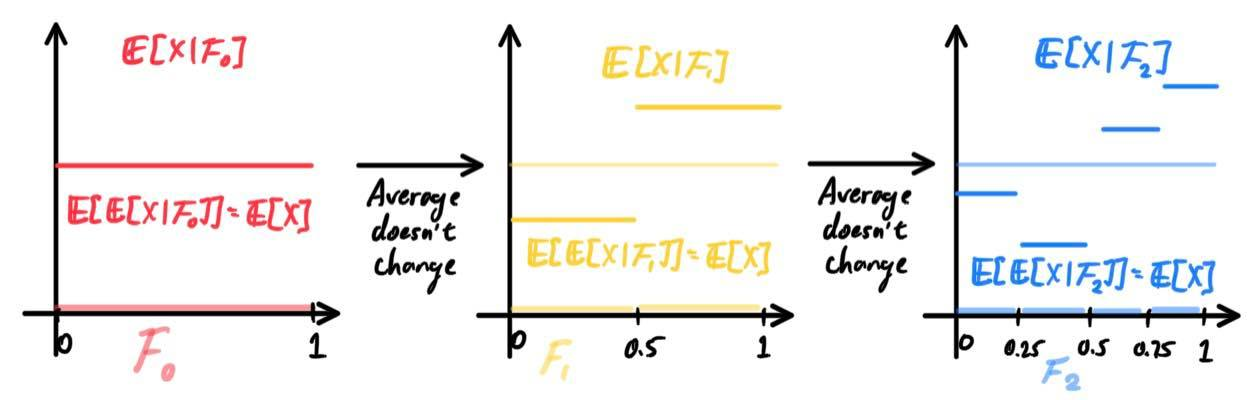
\includegraphics[scale=0.3]{img/martingale_increments.jpg}
  \end{center}
  
  A supermartingale (and submartingale) just means that as we make the function finer and finer, its mean goes down (or up). 


  Martingales are used to model lots of random walk events. In the following three examples, let $\xi_1, \xi_2, \ldots$ be iid, and let $S_n = S_0 + \xi_1 + \ldots + \xi_n$., where $S_0$ is a constant. Let $\mathcal{F}_n = \sigma(\xi_1, \ldots, \xi_n)$ for $n \geq 1$ and let $\mathcal{F}_0 = \{\emptyset, \Omega\}$. 

  \begin{example}[Linear Martingale]
    Let $\mu = \mathbb{E}[\xi_i] = 0$. Then, $\{S_n\}$ is a martingale with respect to $\mathcal{F}_n$. We show the three requirements: 
    \begin{enumerate}
      \item $\mathbb{E}[S_n] = \mathbb{E}[S_0] + \mathbb{E}[\xi_1] + \ldots + \mathbb{E}[\xi_n] = S_0 < \infty$. 
      
      \item By definition, we know that $\xi_i$ is $\sigma(\xi)$-measurable for all $i \in [n]$, so $\xi_i$ is $\mathcal{F}_n = \sigma(\xi_1, \ldots, \xi_n)$-measurable. Since the set of $\mathcal{F}_n$-measurable functions has a vector space structure, $S_n$ is also $\mathcal{F}_n$-measurable. 
      
      \item We can simply solve 

        \[\mathbb{E}[S_{n+1} \mid \mathcal{F}_n] = \mathbb{E}[S_n \mid \mathcal{F}_n] + \mathbb{E}[\xi_{n+1} \mid \mathcal{F}_n] = X_n + \mathbb{E}[\xi_{n+1}] = X_n\]

      where the first equality follows from linearity. For the second equality, note that $S_n$ is $\mathcal{F}_n$-measurable from above, and so the best $\mathcal{F}_n$-measurable approximation of $X$ is $X$ itself (i.e. we have complete information). We know that $\xi_{n+1}$ is independent of the $\xi_i$'s, and so by definition their $\sigma$-algebras are independent. This implies that $\sigma(\xi_{n+1})$ and $\mathcal{F}_n = \sigma(\xi_1, \ldots, \xi_n)$ are independent, and so due to irrelevant information, $\mathbb{E}[\xi_{n+1} \mid \mathcal{F}_n] = \mathbb{E}[\xi_{n+1}]$. 
    \end{enumerate}
    If $\mu \leq 0$ or $\mu \geq 0$, then the computation above shows that $\mathbb{E}[S_{n+1} \mid \mathcal{F}_n] \leq 0$ or $\mathbb{E}[S_{n+1} \mid \mathcal{F}_n] \geq 0$, making it a supermartingale or submartingale, respectively. 
  \end{example}

  Given a supermartingale or submartingale, we can change it to be a martingale. 

  \begin{example}
  Given that $\mu = \mathbb{E}[\xi_i] \neq 0$, then $\{S_n - n\mu\}$is a martingale with respect to $\mathcal{F}_n$. We can see this because

  \begin{align*}
    \mathbb{E}[S_{n+1} - (n + 1)\mu \mid \mathcal{F}_n] & = \mathbb{E}[S_n - n \mu \mid \mathcal{F}_n] + \mathbb{E}[\xi_{n+1} - \mu \mid \mathcal{F}_n] \\
    & = S_n - n \mu + \mathbb{E}[\xi_{n+1}] - \mu \\
    & = S_n - n
  \end{align*}
  \end{example}

  \begin{example}[Quadratic Martingale]
  Say $\mu = \mathbb{E}[\xi_i] = 0$ and $\sigma^2 = \mathrm{Var}(\xi_i) < \infty$. Then, $\{S_n^2 - n \sigma^2\}$ is a martingale. 

  \begin{align*}
    \mathbb{E}[S_{n+1}^2 - (n + 1) \sigma^2 \mid \mathcal{F}_n] & = \mathbb{E}[ (S_n + \xi_{n+1})^2 - (n _ 1) \sigma^2 \mid \mathcal{F}_n] \\
    & = \mathbb{E}[S^2 - n \sigma^2 \mid \mathcal{F}_n ] + \mathbb{E}[ 2 S_n \xi_{n+1} + \xi_{n+1}^2 - \sigma^2 \mid \mathcal{F}_n] \\
    & = \mathbb{E}[S^2 - n \sigma^2 \mid \mathcal{F}_n ] + 2 \mathbb{E}[ S_n \xi_{n+1} \mid \mathcal{F}_n ] + \mathbb{E}[\xi_{n+1}^2] - \sigma^2  \\
    & = \mathbb{E}[S^2 - n \sigma^2 \mid \mathcal{F}_n ]
  \end{align*}

  where we have used the fact that due to independence of $\xi_{n+1}$ with $\mathcal{F}_n$, we have $\mathbb{E}[S_n \xi_{n+1} \mid \mathcal{F}_n] = \mathbb{E}[S_n \mathbb{E}[ \xi_{n+1} \mid \mathcal{F}_n]] = \mathbb{E}[S_n \cdot 0] = 0$. 
  \end{example}

  This following result shows that martingales with bounded increments either converge or oscillate between $+\infty$ and $-\infty$. 

  \begin{theorem}
    Let $\{X_n\}_{n \in \mathbb{N}}$ be a martingale with $|X_{n+1} - X_n| \leq M < \infty$. Let 

    \begin{align*}
      C & = \{\lim_{n \rightarrow \infty} X_n \text{ exists and is finite}\} \\
      D & = \{\lim_{n \rightarrow \infty} \sup X_n = +\infty \text{ and } \lim_{n \rightarrow \infty} \inf X_n = -\infty\}
    \end{align*}

    Then $\mathbb{P}(C \cup D) = 1$. 
  \end{theorem}

\end{document}
